% \documentclass{article}

\documentclass[conference]{IEEEtran}

% \documentclass[runningheads]{llncs}

\makeatletter
\def\endthebibliography{%
  \def\@noitemerr{\@latex@warning{Empty `thebibliography' environment}}%
  \endlist
}
\makeatother
\pagestyle{plain}
\usepackage{graphics}
\usepackage{hyperref}
\usepackage{amsmath}
% \usepackage{listings}
\usepackage{xspace}
% \usepackage{bigstrut}
\usepackage{booktabs}
\usepackage{subfigure}
\usepackage{url}
\usepackage{mathtools}
\usepackage{amsfonts}
\usepackage{amssymb}
\usepackage{multirow}
% \usepackage[ruled,vlined]{algorithm2e}
% \usepackage{algpseudocode}
\usepackage{enumitem}
\usepackage{numprint}
% \usepackage[normalem]{ulem}
\usepackage{tcolorbox}
\usepackage{xurl}
\usepackage{xstring}
\usepackage[T1]{fontenc}
\usepackage{graphicx}
\usepackage{setspace}
\usepackage{makecell}
% \usepackage{xcolor}
\usepackage{xcolor,colortbl}
% \usepackage[a4paper,
%             bindingoffset=0in,
%             left=2.5cm,,
%             right=2.5cm,
%             top=1.35in,
%             bottom=1.35in,
%             footskip=.25in]{geometry}

% \usepackage{lipsum}
\usepackage{caption}% http://ctan.org/pkg/caption
\usepackage{algorithm}% http://ctan.org/pkg/algorithm
\usepackage{algpseudocode}% http://ctan.org/pkg/algorithmicx
% \usepackage{algorithmic}  
% \usepackage[algo2e]{algorithm2e} 
% \usepackage[n,landau,notions,ff,mm]{cryptocode}

% \usepackage{pifont}
\usepackage{wasysym}

% Define custom colors
\definecolor{gainsboro}{rgb}{0.86, 0.86, 0.86}
\definecolor{forest}{rgb}{0.86, 0.86, 0.86}
\definecolor{lightbrown}{rgb}{0.91, 0.94, 0.82} 
\definecolor{lightgray}{rgb}{0.93, 0.93, 0.93} 

\definecolor{lightblue}{rgb}{0.9, 0.9, 0.93} 

\definecolor{CustomColor1}{RGB}{200, 217, 237} % Example light blue
\definecolor{CustomColor2}{RGB}{196, 225, 165} % Example light green
\definecolor{CustomColor3}{RGB}{255, 213, 179} % Example light orange

\definecolor{backgroundcolor}{RGB}{242, 248, 255}

% \newcommand{\rui}[1]{{\color{orange} #1}}
\newcommand{\rui}[1]{{\color{black} #1}}

\usepackage{graphicx} % Required for inserting images
\usepackage{hyperref}
\hypersetup{
    colorlinks=true,
    linkcolor=blue,
    filecolor=magenta,      
    urlcolor=cyan,
    % pdftitle={Overleaf Example},
    pdfpagemode=FullScreen,
}
\usepackage{amsmath}

\usepackage{xcolor} % Add this in your preamble


\usepackage{rotating}

\usepackage{afterpage}
\usepackage{todonotes}
\setuptodonotes{inline, color=blue!30}

\usepackage[framemethod=TikZ]{mdframed}
\usepackage{algorithm}
\usepackage{algpseudocode}

\usepackage{acro}
\acsetup{single}


\DeclareAcronym{ZKP}{
  short = ZKP,
  long  = Zero-knowledge proof,
}
\newcommand{\ZKP}{\ac{ZKP}\xspace}

\DeclareAcronym{FL}{
  short = FL,
  long  = Federated Learning,
}
\newcommand{\FL}{\ac{FL} Alliance\xspace}


% \DeclareAcronym{SNT}{
%   short = SNT,
%   long  = Single Node Training,
% }
% \newcommand{\SNT}{\ac{SNT}\xspace}


\newcommand{\SNT}{{AI Arena}\xspace}

\DeclareAcronym{VRF}{
  short = VRF,
  long  = Verifiable Random Function,
}
\newcommand{\VRF}{\ac{VRF}\xspace}


\DeclareAcronym{DeFi}{
  short = DeFi,
  long  = Decentralized Finance,
}
\newcommand{\DeFi}{\ac{DeFi}\xspace}

% \DeclareAcronym{PGA}{
%   short = PGA,
%   long  = Priority Gas Auction,
% }
% \newcommand{\PGA}{\ac{PGA}\xspace}
% \newcommand{\PGAs}{\acp{PGA}\xspace}

\DeclareAcronym{PoW}{
  short = PoW,
  long  = Proof-of-Work,
}
\newcommand{\PoW}{\ac{PoW}\xspace}

\DeclareAcronym{PoS}{
  short = PoS,
  long  = Proof-of-Stake,
}
\newcommand{\PoS}{\ac{PoS}\xspace}

\DeclareAcronym{LTVV}{
  short = LTV,
  long  = Loan-to-Value,
}
\newcommand{\LTVV}{\ac{LTVV}\xspace}



\DeclareAcronym{LLM}{
  short = LLM,
  long  = Large Language Model,
}
\newcommand{\LLM}{\ac{LLM}\xspace}
\newcommand{\LLMs}{\acp{LLM}\xspace}

\DeclareAcronym{APR}{
  short = APR,
  long  = Annual Percentage Rate,
}
\newcommand{\APR}{\ac{APR}\xspace}
\newcommand{\APRs}{\acp{APR}\xspace}

\DeclareAcronym{ROI}{
  short = ROI,
  long  = Return On Investment,
}
\newcommand{\ROI}{\ac{ROI}\xspace}

\DeclareAcronym{NRF}{
  short = NRF,
  long  = Nearly Risk-Free,
}
\newcommand{\NRF}{\ac{NRF}\xspace} 

\DeclareAcronym{IL}{
  short = IL,
  long  = Impermanent Loss,
}
\newcommand{\IL}{\ac{IL}\xspace} 


\DeclareAcronym{RL}{
  short = RL,
  long  = Realized Loss,
}
\newcommand{\RL}{\ac{RL}\xspace} 



\DeclareAcronym{PNL}{
  short = PNL,
  long  = Profit and Loss,
}
\newcommand{\PNL}{\ac{PNL}\xspace} 
\newcommand{\PNLs}{\acp{PNL}\xspace}


\DeclareAcronym{JIT}{
  short = JIT,
  long  = Just-in-Time,
}
\newcommand{\JIT}{\ac{JIT}\xspace}
\newcommand{\JITs}{\acp{JIT}\xspace}

\DeclareAcronym{LP}{
  short = LP,
  long  = Liquidity Provider,
}
\newcommand{\LP}{\ac{LP}\xspace}
\newcommand{\LPs}{\acp{LP}\xspace}

\DeclareAcronym{LT}{
  short = LT,
  long  = Liquidity Taker,
}
\newcommand{\LT}{\ac{LT}\xspace}
\newcommand{\LTs}{\acp{LT}\xspace}

\DeclareAcronym{NO}{
  short = NO,
  long  = Node Operator,
}
\newcommand{\NO}{\ac{NO}\xspace}
\newcommand{\NOs}{\acp{NO}\xspace}


\DeclareAcronym{LSD}{
  short = LSD,
  long  = Liquid Staking Derivative,
}
\newcommand{\LSD}{\ac{LSD}\xspace}
\newcommand{\LSDs}{\acp{LSD}\xspace}

\DeclareAcronym{LST}{
  short = LST,
  long  = Liquid Staking Tokens,
}
\newcommand{\LST}{\ac{LST}\xspace}
\newcommand{\LSTs}{\acp{LST}\xspace}


\DeclareAcronym{DEX}{
  short = DEX,
  long  = Decentralized Exchange,
}
\newcommand{\DEX}{\ac{DEX}\xspace}
\newcommand{\DEXes}{\acp{DEX}\xspace}

\DeclareAcronym{CEX}{
  short = CEX,
  long  = Centralized Exchange,
}
\newcommand{\CEX}{\ac{CEX}\xspace}
\newcommand{\CEXes}{\acp{CEX}\xspace}

\DeclareAcronym{EOA}{
  short = EOA,
  long  =  Externally-Owned Account,
}
\newcommand{\EOA}{\ac{EOA}\xspace}
\newcommand{\EOAs}{\acp{EOA}\xspace}


\DeclareAcronym{NFT}{
  short = NFT,
  long  = Non-fungible Token,
}
\newcommand{\NFT}{\ac{NFT}\xspace}
\newcommand{\NFTs}{\acp{NFT}\xspace}

% \DeclareAcronym{LP}{
%   short = LP,
%   long  = Liquidity Provider,
% }
% \newcommand{\LP}{\ac{LP}\xspace}
% \newcommand{\LPs}{\acp{LP}\xspace}


\DeclareAcronym{P2P}{
  short = P2P,
  long  = Peer-to-Peer,
}
\newcommand{\PtP}{\ac{P2P}\xspace}

\DeclareAcronym{TVL}{
  short = TVL,
  long  = Total Value Locked,
}
\newcommand{\TVL}{\ac{TVL}\xspace}


\DeclareAcronym{CFMM}{
  short = CFMM,
  long  = Constant Function Market Maker,
}
\newcommand{\CFMM}{\ac{CFMM}\xspace}

\DeclareAcronym{CPMM}{
  short = CPMM,
  long  = Constant Product Market Maker,
}
\newcommand{\CPMM}{\ac{CPMM}\xspace}


\DeclareAcronym{DApp}{
  short = DApp,
  long  = Decentralized Application,
}
\newcommand{\DApp}{\ac{DApp}\xspace}
\newcommand{\DApps}{\acp{DApp}\xspace}

\DeclareAcronym{DAO}{
  short = DAO,
  long  = Decentralized Autonomous Organisation,
}
\newcommand{\DAO}{\ac{DAO}\xspace}
\newcommand{\DAOs}{\acp{DAO}\xspace}


\DeclareAcronym{CeFi}{
  short = CeFi,
  long  = Centralized Finance,
}
\newcommand{\CeFi}{\ac{CeFi}\xspace}

\DeclareAcronym{MEV}{
  short = MEV,
  long  = Miner Extractable Value,
}
\newcommand{\MEV}{\ac{MEV}\xspace}

\DeclareAcronym{EV}{
  short = EV,
  long  = Extractable Value,
}
\newcommand{\EV}{\ac{EV}\xspace}

\DeclareAcronym{BEV}{
  short = BEV,
  long  = Blockchain Extractable Value,
}
\newcommand{\BEV}{\ac{BEV}\xspace}


\DeclareAcronym{AMM}{
  short = AMM,
  long  = Automated Market Maker,
}
\newcommand{\AMM}{\ac{AMM}\xspace}
\newcommand{\AMMs}{\acp{AMM}\xspace}

\DeclareAcronym{FaaS}{
  short = FaaS,
  long  = Front-running as a Service,
}
\newcommand{\FaaS}{\ac{FaaS}\xspace}

\DeclareAcronym{SaaS}{
  short = SaaS,
  long  = Staking as a Service,
}
\newcommand{\SaaS}{\ac{SaaS}\xspace}
\newcommand{\SaaSs}{\acp{SaaS}\xspace}

\DeclareAcronym{HFT}{
  short = HFT,
  long  = High-frequency Trading,
}
\newcommand{\HFT}{\ac{HFT}\xspace}


\DeclareAcronym{PGA}{
  short = PGA,
  long  = Priority Gas Auction,
}
\newcommand{\PGA}{\ac{PGA}\xspace}
\newcommand{\PGAs}{\acp{PGA}\xspace}

\DeclareAcronym{BRF}{
  short = BRF,
  long  = Back-run Flodding,
}
\newcommand{\BRF}{\ac{BRF}\xspace}

\DeclareAcronym{PRG}{
  short = PRG,
  long  = Priority Gas Auction,
}
\newcommand{\PRG}{\ac{PRG}\xspace}

%% design patterns
\DeclareAcronym{AE}{
  short = AE,
  long  = Atomic Execution,
}
\newcommand{\AEE}{\ac{AE}\xspace}


\DeclareAcronym{BEET}{
  short = BEET,
  long  = Break-even Extraction Threshold,
}
\newcommand{\BEET}{\ac{BEET}\xspace}


\DeclareAcronym{BAD}{
  short = BAD,
  long  = Breaking Atomicity and Determinism,
}
\newcommand{\BAD}{\ac{BAD}\xspace}

%% novel design

\DeclareAcronym{aamm}{
  short = A$^2$MM,
  long  = Automated Arbitrage Market Maker,
}
\newcommand{\aamm}{\ac{aamm}\xspace}


\DeclareAcronym{dfmm}{
  short = DFMM,
  long  = Dynamic Fee Market Maker,
}
\newcommand{\dfmm}{\ac{dfmm}\xspace}

\DeclareAcronym{dfaamm}{
  short = A$^2_F$MM,
  long  = Automated Arbitrage and Fee Market Maker,
}
\newcommand{\dfaamm}{\ac{dfaamm}\xspace}


\DeclareAcronym{MVI}{
  short = MVI,
  long  = Minimum Victim Input,
}
\newcommand{\MVI}{\ac{MVI}\xspace}


\DeclareAcronym{BSC}{
  short = BSC,
  long  = Binance Smart Chain,
}
\newcommand{\BSC}{\ac{KS}\xspace}

\DeclareAcronym{KS}{
  short = KS,
  long  = Kolmogorov-Smirnov,
}
\newcommand{\KS}{\ac{KS}\xspace}


\newcommand{\FML}{\ensuremath{\xspace\texttt{FML}}\xspace}



%coins
\newcommand{\coins}{\ensuremath{\xspace\texttt{coin}}\xspace}
% \newcommand{\ETH}{\ensuremath{\xspace\texttt{ETH}}\xspace}
\newcommand{\DAI}{\ensuremath{\xspace\texttt{DAI}}\xspace}
\newcommand{\USDC}{\ensuremath{\xspace\texttt{USDC}}\xspace}
\newcommand{\BNB}{\ensuremath{\xspace\texttt{BNB}}\xspace}
\newcommand{\BTC}{\ensuremath{\xspace\texttt{BTC}}\xspace}
\newcommand{\USD}{\ensuremath{\xspace\texttt{USD}}\xspace}
\newcommand{\USDT}{\ensuremath{\xspace\texttt{USDT}}\xspace}
\newcommand{\fUSDC}{\ensuremath{\xspace\texttt{fUSDC}}\xspace}
\newcommand{\WBTC}{\ensuremath{\xspace\texttt{WBTC}}\xspace}
\newcommand{\renBTC}{\ensuremath{\xspace\texttt{renBTC}}\xspace}
\newcommand{\KYL}{\ensuremath{\xspace\texttt{KYL}}\xspace}
\newcommand{\WETH}{\ensuremath{\xspace\texttt{WETH}}\xspace}

\newcommand{\NPXS}{\ensuremath{\xspace\texttt{NPXS}}\xspace}
\newcommand{\BNT}{\ensuremath{\xspace\texttt{BNT}}\xspace}
\newcommand{\XRP}{\ensuremath{\xspace\texttt{XRP}}\xspace}

\newcommand{\stETH}{\ensuremath{\xspace\texttt{stETH}}\xspace}

\newcommand{\sfraxETH}{\ensuremath{\xspace\texttt{sfraxETH}}\xspace}

\newcommand{\fraxETH}{\ensuremath{\xspace\texttt{fraxETH}}\xspace}

\newcommand{\ETH}{\texttt{ETH}\xspace}
\newcommand{\rETH}{\texttt{rETH}\xspace}
\newcommand{\frxETH}{\texttt{frxETH}\xspace}
\newcommand{\sfrxETH}{\texttt{sfrxETH}\xspace}
\newcommand{\sETHt}{\texttt{sETH2}\xspace}
\newcommand{\rETHt}{\texttt{rETH2}\xspace}

\newcommand{\tx}{\mathsf{tx}\xspace}


\newcommand{\totalSupply}{\ensuremath{\xspace\color{brown}\mathsf{X_{totalSupply}}}\xspace}
\newcommand{\initialEmission}{\ensuremath{\xspace\color{brown}\mathsf{X_{initialEmission} }}\xspace}

\newcommand{\overTimeEmission}{\ensuremath{\xspace\color{brown}\mathsf{X_{overTimeEmission} }}\xspace}

\newcommand{\dailyEmission}{\ensuremath{\xspace\color{brown}\mathsf{X_{dailyEmission} }}\xspace}



\title{FLock: Federated Machine Learning on Blockchain \\ \vspace{0.5cm}\large 
Democratising AI through Decentralisation of Data, Computation, and Models
}
\author{\texttt{FLock Team}}
% \date{\today}

\usepackage{fancyhdr}
\pagestyle{fancy}
\fancyhf{}  % Clear header and footer
\chead{FLock: Federated Machine Learning on Blockchain (Version \today)}
\cfoot{\thepage}
\renewcommand{\headrulewidth}{0pt}
\renewcommand{\footrulewidth}{0pt}

\begin{document}
\pagecolor{backgroundcolor}
\maketitle
\thispagestyle{empty}

\begin{abstract}
 The rapid pace of AI development has highlighted significant challenges in its creation and deployment, primarily due to the centralised control maintained by a few large corporations. Such an approach exacerbates biases within AI models due to a lack of effective governance and oversight. Furthermore, it diminishes public engagement and raises serious data protection concerns. The resulting monopolistic control over data and model outputs also poses a threat to innovation and equitable data usage, as users unknowingly contribute to data sets that serve the interests of these corporations.

 FLock democratises AI development and alignment through on-chain incentive mechanisms. By promoting open source development and data ownership, FLock facilitates an open and collaborative environment where participants can contribute models, data, and computing resources with rewards determined by on-chain consensus. This approach improves transparency and collaboration at scale without introducing biases from centralised entities. Ultimately, FLock enables diverse communities to develop purpose-built AI models, offering bespoke solutions tailored to their specific needs, revolutionising the landscape of AI development and deployment.
 
\end{abstract}

\section{Introduction}

Spanning all fields, collaboration has historically catalysed innovation. This is manifest in the case of the scientific and the digital. By pooling collective expertise, we have forged disruptive solutions at speed. At present, this ideal faces barriers when applied to AI development and deployment: notably, diminished public engagement, pervasive concerns regarding concentrated control, and data protection exerted by a handful of corporations. Meanwhile, blockchain technology~\cite{nakamoto2008bitcoin, wood2014ethereum} has demonstrated its efficacy in multiple areas needing distributed corporations, such as decentralized finance~\cite{werner2022sok}, voting and governance. Research into and deployment of blockchain to transform AI development is now underway. 

FLock, predicated on community involvement and a staunch commitment to data protection, is poised to spearhead the democratisation of AI ecosystem by using blockchain.


\begin{figure}[t]
\centering
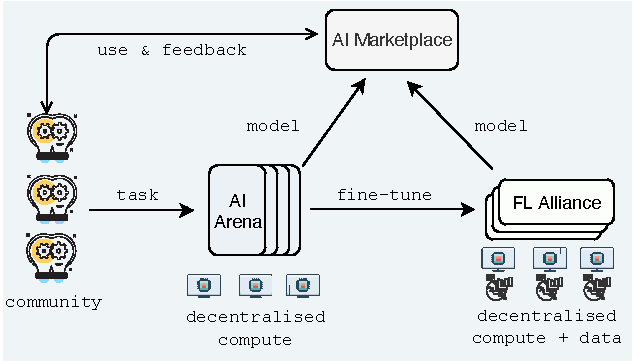
\includegraphics[width=\columnwidth]{figures/flock-snt-fl.pdf}
\caption{FLock System Logic. Upon a task creation, the model is first trained and validated in AI Arena, a blockchain-based decentralised training platform, and then optionally further fine-tuned in FL Alliance using participants' local data. Finally, the model is deployed by applications in the AI Marketplace, where feedback will be used to further improve the model.}
\label{fig:FLock-system-logic}
\end{figure}

\subsection{The Problems with Centralised Control over AI Creation}
In the present day, the primary obstacle to innovation in the realm of AI is its centralised control. This centralised structure mandates that all AI training, decision-making processes, and data storage are controlled within a single entity or location~\cite{bellavista2021decentralised}. 
This results in the following pitfalls:
\begin{description}
    \item \textbf{Single Point of Failure:} Vulnerability to disruptions from technical issues and cyberattacks.
    \item \textbf{Value Plurality}: Lack of value plurality means biases of single entities are reflected in AI. With centralised institutions exerting absolute control over models~\cite{wu2023brief, shen2024hugginggpt}, the values of the output models are also centralised~\cite{anil2023palm}. For instance, the world reimagined by Google’s generative AI tool, Gemini, is widely criticised~\cite{gemini-wont-show-you-white-people}.

    \item \textbf{Data Protection:} Providers of closed-source \LLMs~\cite{zhao2023survey}, such as \href{https://openai.com/}{OpenAI}, have the capability to monitor all user interactions with their models, thereby raising significant data protection concerns. In addition, under this centralised framework, every user who interacts with a \LLM becomes an unwitting contributor of data to these vast corporations that maintain ownership of the models. There is a pressing need to enhance the fairness of contribution incentives and to more accurately assess the value of user-contributed data.

    \item \textbf{Governance:} Recent research~\cite{nist-report,IBM-report,MIT-report} has highlighted a concerning trend in which the lack of governance has led to a pronounced exacerbation of biases and inaccuracies within the models.

    \item \textbf{Scalability:} As the volume of data and complexity of tasks increase, limited processing power acts as a bottleneck.

    \item \textbf{Innovation:} Progress is stifled in an environment where a limited number of entities have the means to experiment.
\end{description}


\begin{figure*}[t]
\centering
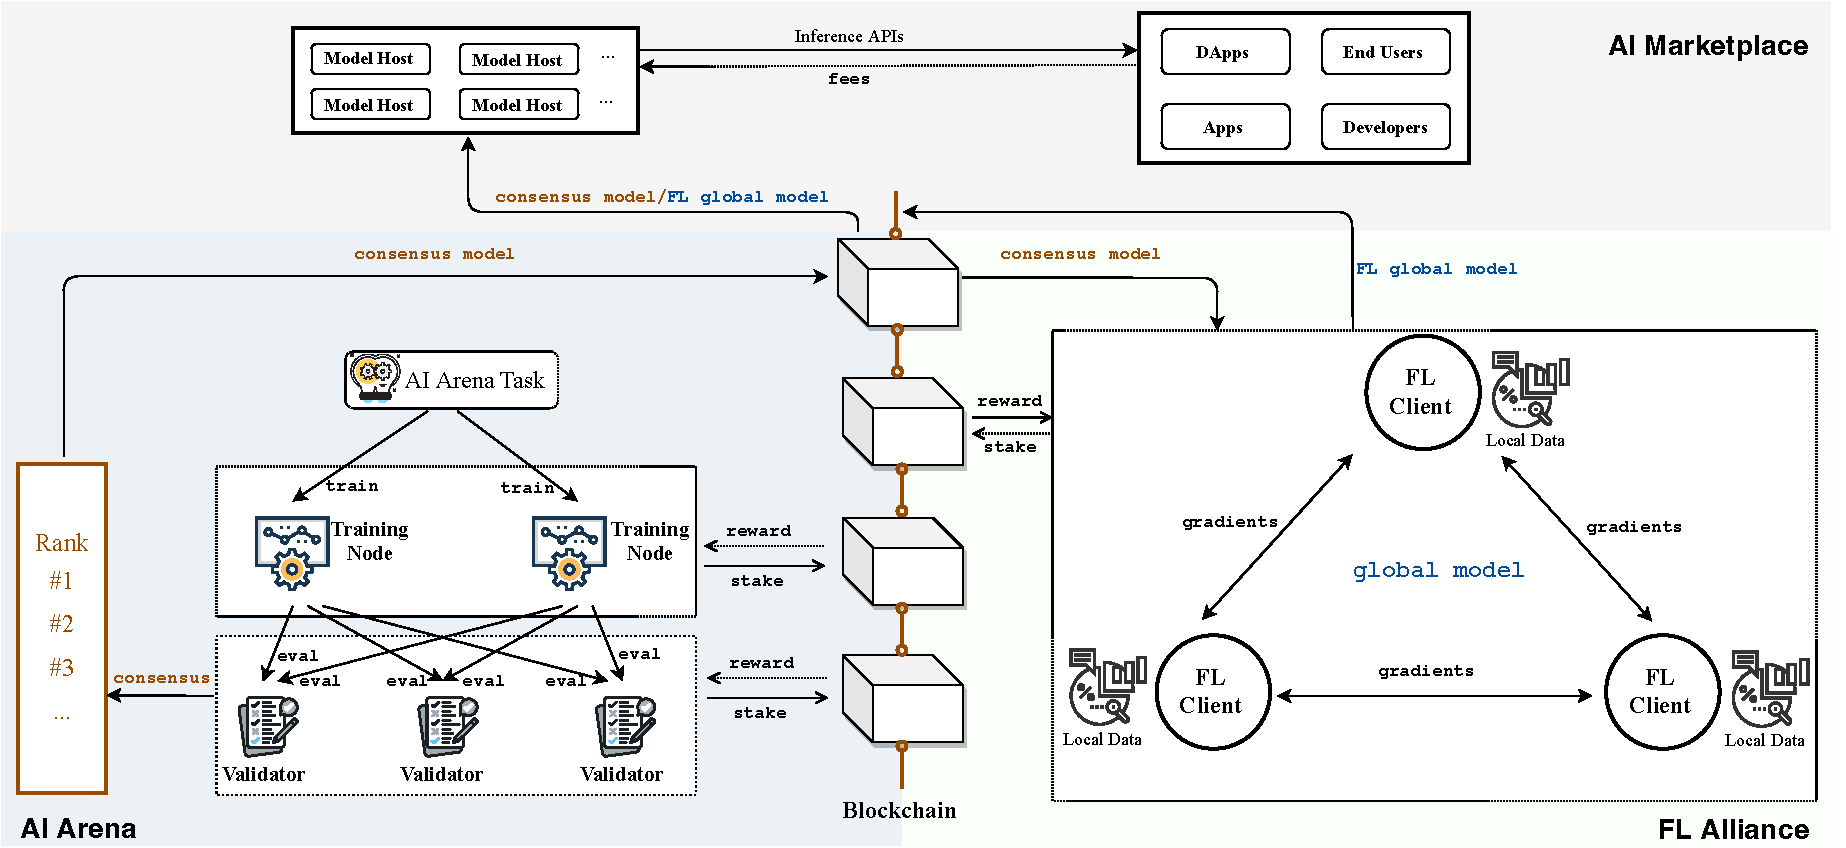
\includegraphics[width=2\columnwidth]{figures/flock-system-overview_simplified.pdf}
\caption{FLock System Overview. When a task is created in AI Arena, it is first trained by training nodes. These nodes then submit their models to validators, who evaluate and propose scores for each submission. The validators reach a consensus on these scores to determine the ranking of the submitted models. The consensus model can then be assigned to FL clients, who fine-tune and improve it using their local data, resulting in the FL global model. The AI Arena consensus model or the FL global model can be deployed and hosted in the AI Marketplace, providing interfaces to various applications. AI Arena train nodes, validators and FL clients need to stake to participate the system, and will be rewarded based on their performance.}
\label{fig:FLock-system}
\end{figure*}


\subsection{FLock's Solution}



% \begin{figure}[t]
% \centering
% \includegraphics[width=\columnwidth]{figures/FLock-logic.pdf}
% \caption{FLock System Logic.}
% \label{fig:FLock-system-logic}
% \end{figure}

FLock~\cite{dong2022FLock,dong2023defending} is a blockchain-based platform for decentralised AI.  As shown in Figure~\ref{fig:FLock-system-logic} and~\ref{fig:FLock-system}, FLock eliminates obstacles that prevent active participation in AI systems, empowering communities to contribute models, data, or computing resources in a modular and decentralised way. AI models can be trained and validated in \SNT and further refined in \FL. Harnessing blockchain technology, FLock introduces incentive mechanisms for participants, fostering a collaborative environment. This results in the development of a wide range of purpose-built models, created by, with, and for the communities, offering tailored solutions to meet specific needs.


% This whitepaper outlines a visionary direction for advancing AI through decentralised collaborative efforts incentivised by on-chain rewards. It lays out the formidable barriers stifling AI development in the present day. Next, it presents how systems and mechanisms such as those developed by FLock offer a promising and sustainable solution.



% \subsection{How Web3 Can Transform AI?}

% % \begin{figure*}[t]
% % \centering
% % 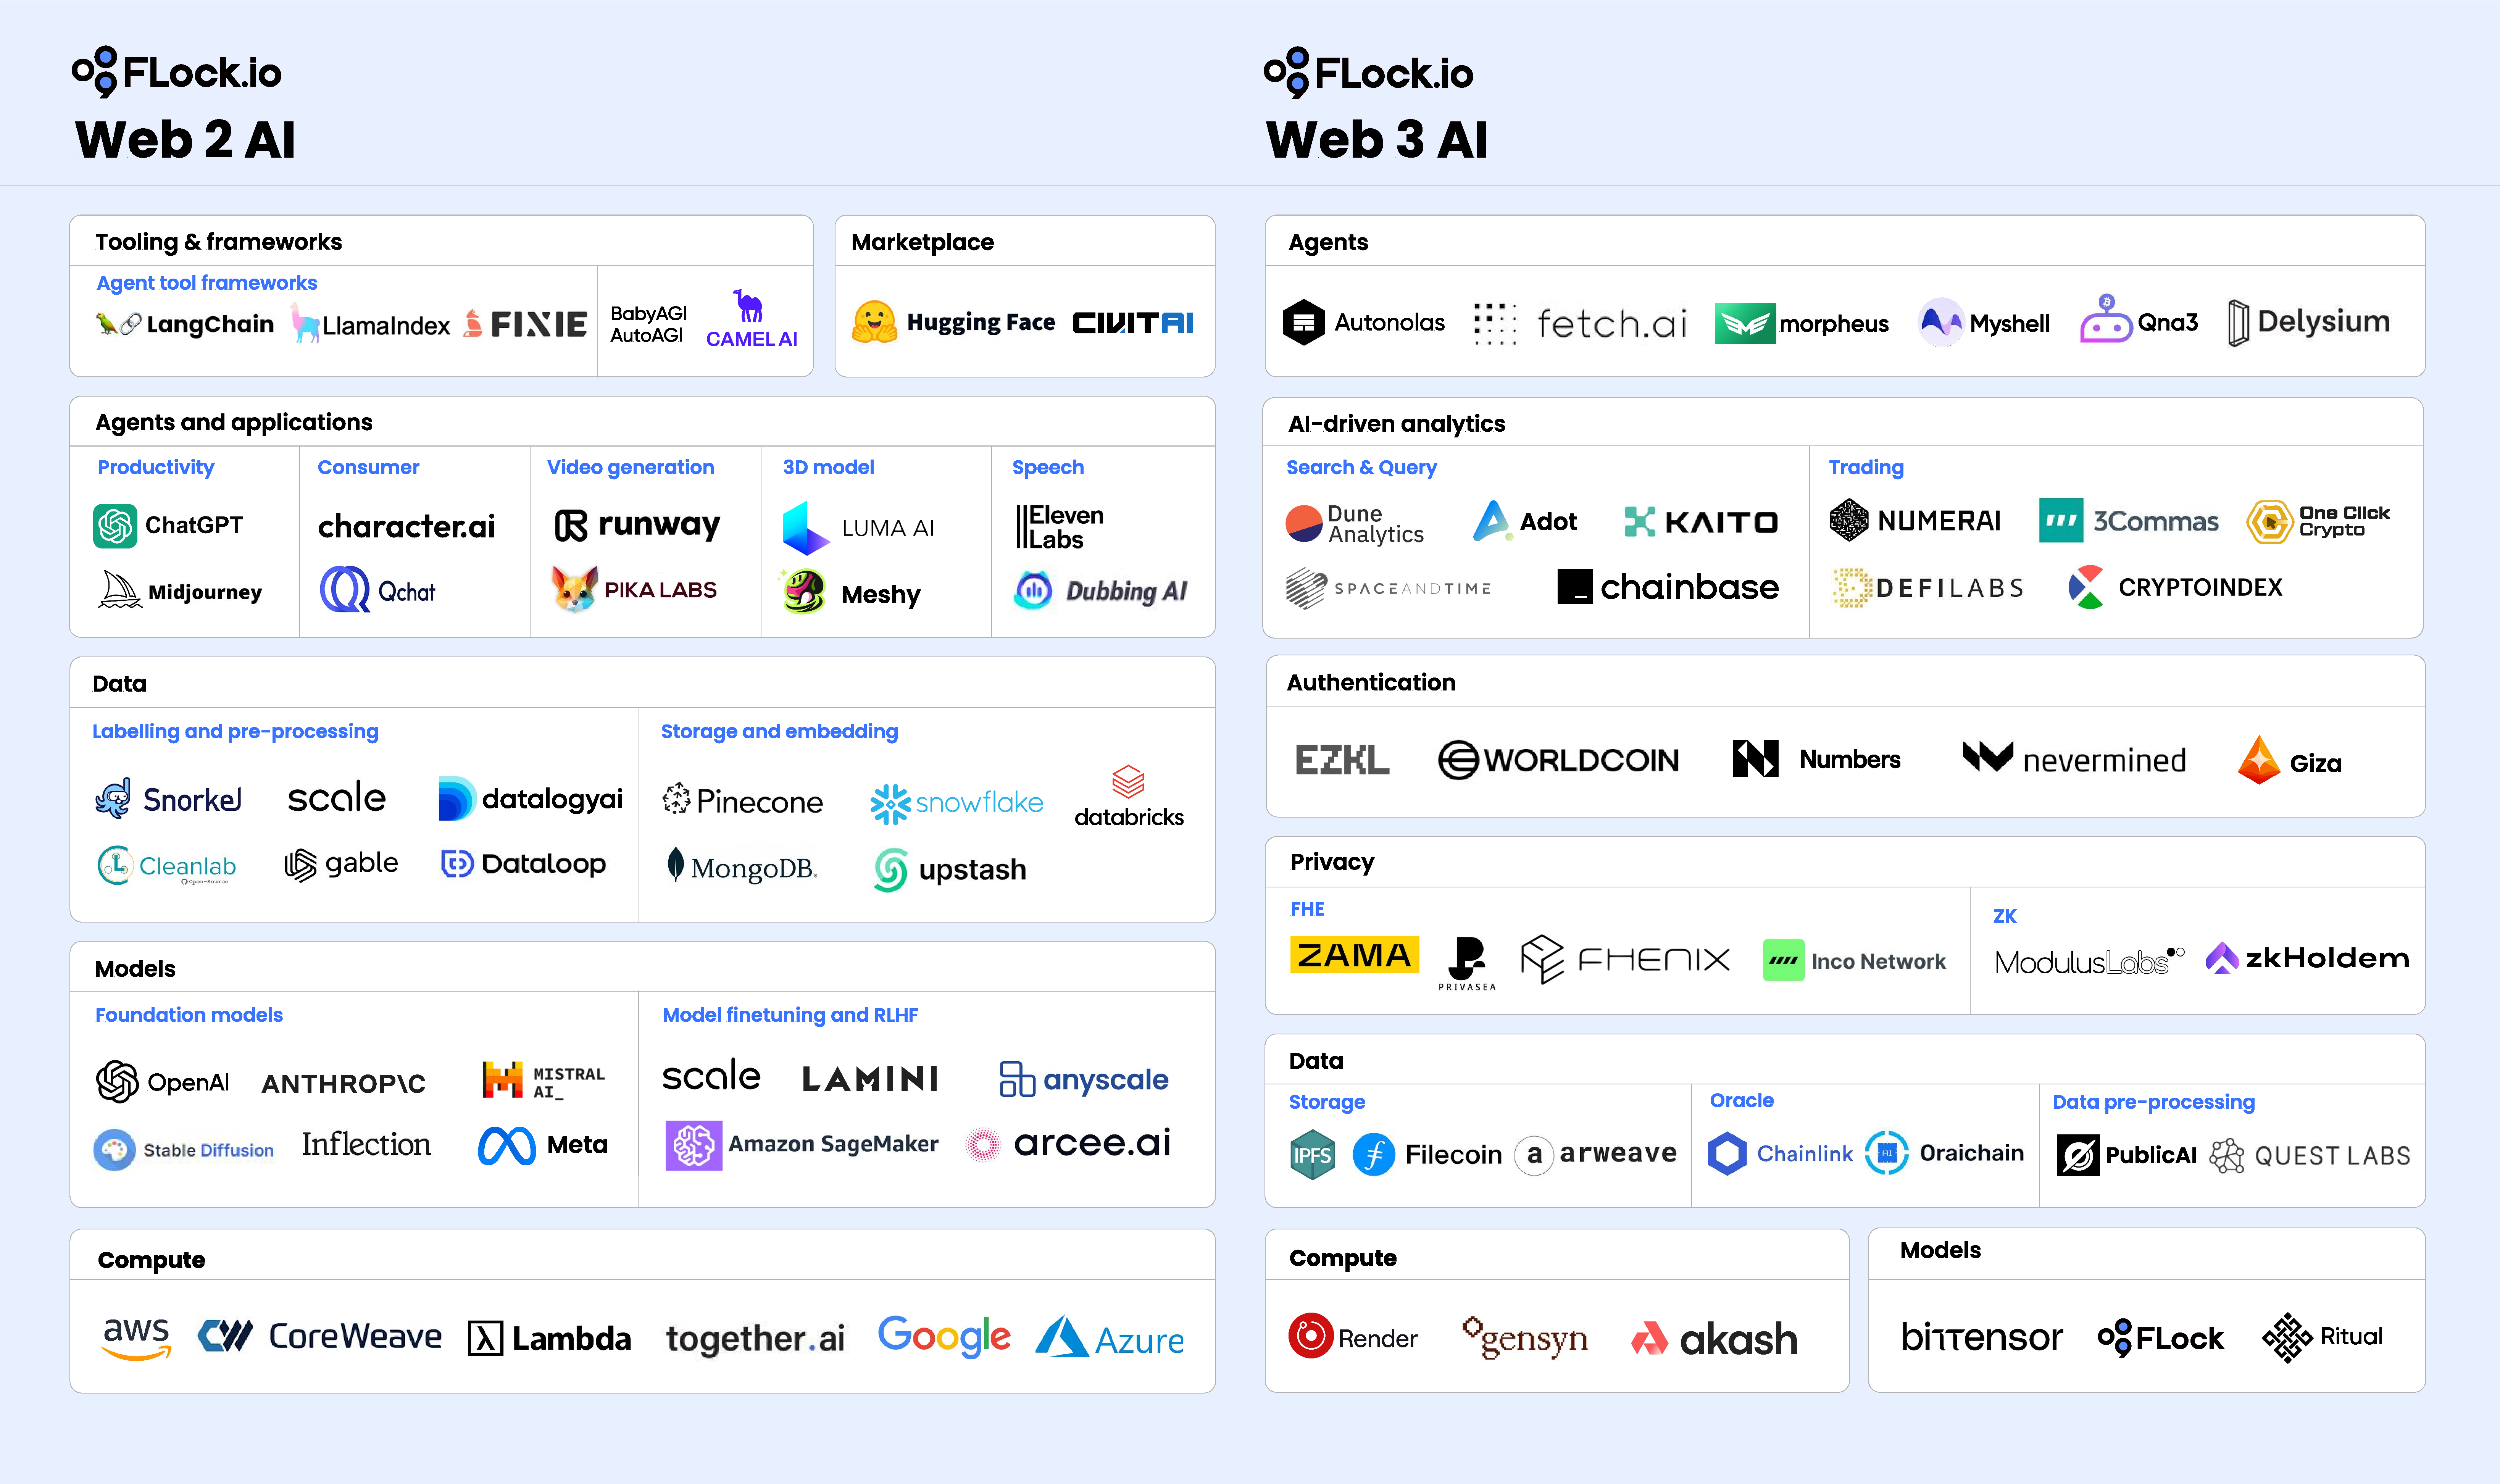
\includegraphics[width=2\columnwidth]{figures/web2 and web3 Mapping.pdf}
% % \caption{AI Project Landscape in Web 2 and Web 3.}
% % \label{fig:AI_project_landscape}
% % \end{figure*}
% % \todo{@Frank extend the related work}

% Transitioning into Web3 involves enhanced data protection and authentication for heightened security and transparency. Decentralisation allows trust, ownership, and innovation to thrive.
% % as shown in Figure~\ref{fig:AI_project_landscape}.
% \begin{itemize}
%  \item  {\textbf{Decentralised Compute. }}Blockchains are facilitating the shift from from centralised cloud services like Azure, AWS to a decentralised network of global resources. This way, participants can contribute computational power to form a network without a single point of failure.

%  \item  {\textbf{Model Development. }}Unlike centralised platforms like OpenAI that dominated Web2, Web3 embraces decentralised model construction, which facilitates collective contributions from a global community.

%  \item  {\textbf{Data Democratisation. }}Web3 effaces the presently dominating framework that locks data in corporate vaults, and replaces it with a progressive social contract that permits the public and independent developers to annotate data for new research, from medical analysis to self-driving car training. Distributed storage grants individuals control over their data and rewards them for their contributions.

%  \item  {\textbf{Data Protection. }}Blockchain becomes the shield for your information. Imagine training AI on sensitive medical data without exposing patient identities, thanks to advanced encryption and zero-knowledge proofs. This is Web3’s promise: AI that learns and grows, yet keeps your data safe and under your control.
 
%  % Companies like ZAMA and ModulusLabs are leading the charge, shifting the paradigm from invasive, centralised models to data protection-first AI. 

%  % like EZKL and Worldcoin

%  \item  {\textbf{Authentication. }}Existing Web3 Solutions offer secure, self-sovereign identity management, eliminating the need for centralised platforms to hold your login credentials. This empowers you to log into AI applications without relying on Facebook or Google, enhancing security and putting you in the driver's seat of your digital identity.

% % like Dune Analytics and NumerAI 
%  \item  {\textbf{AI-Driven Analytics. }} Existing Web3 platforms utilise cutting-edge AI algorithms to transform data analysis in Web3. Users can seamlessly explore complex DeFi protocols, identify investment opportunities, and make informed decisions, all powered by AI in a transparent and community-driven ecosystem.

% % like Autonolas and Fetch.ai

%  \item  {\textbf{Decentralised Agents. }}Web3 promotes the development of intelligent agents capable of navigating decentralised networks and autonomously executing tasks on your behalf. These AI agents have the power to manage your investments, negotiate decentralised deals, or optimise your resource allocation across Web3 protocols, unlocking a new era of automation and personalised services.
% \end{itemize}


% \thispagestyle{fancy}
\section{FLock System Overview}
The FLock system consists of the blockchain layer, AI layer, and various participants. Each component plays an essential role in ensuring the system's functionality and security.





\subsection{Blockchain Layer}
FLock's tokenomics incorporates a blockchain-based reward mechanism designed to enhance resilience against malicious user attacks.  This robust security feature is underpinned by a carefully designed incentive mechanism.
The blockchain layer acts as the foundation for both stakeholder participation and the distribution of rewards. This layer employs smart contracts to ensure that participants can securely lock in their stakes, fostering an environment of trust and transparency. The process is designed to incentivise participation by allocating rewards based on contributions, thus encouraging a more engaged and active community.

The blockchain layer's inherent security features safeguard against fraudulent activities, ensuring uncompromised integrity of staking and reward distribution. It is an critical component to support the model safety and improve resilience against malicious user attacks. By leveraging smart contracts, the system automates an efficient and fair rewards process. Automation reduces human error and ensures that rewards are distributed in a timely and fair manner. 

\subsection{AI Layer}

% \subsubsection{Single Node Training}
% \todo{@Ray, Can you please briefly introduce the workflow of Single Node Training in FLock?}

% \subsubsection{Federated Learning}
% \todo{@Ray, Can you please briefly introduce the workflow of FL in FLock?}











The AI layer offers infrastructure for decentralised training, extracting and monetising knowledge from data. It encourages compute and data contributions from the community, using blockchain for rewards based on thier contributions.

\begin{itemize}
    \item {\textbf{\SNT.}} AI layer supports a conventional machine learning~(ML) model training paradigm, optimising models directly on users' devices with their own or public data. To maximise the generalisation ability and performance of the final trained models, this layer is designed to encourage community members to contribute various public or local data, harnessing the broader community's power. By leveraging blockchain, it ensures contributors are continually engaged and rewarded based on the quantifiable impact of their data on improving the models.

 \item  {\textbf{\FL.}} Utilising the FL~\cite{mcmahan2017communication} approach, the AI layer enables thousands of participants to collaboratively train a global model, where data sovereignty is preserved by ensuring that no local data are transmitted at any stage of the training process. Within the AI layer, a model aggregation component allows participants to upload weights from models trained on their unique local data. These weights are then aggregated to build an optimal global model, enhancing its generalisation capabilities and performance. The integration of training task automation and deployment orchestration components simplifies the process for users to join tasks and contribute valuable knowledge extracted from their data.



 % \item \textbf{Connecting \SNT and \FL.} As shown in Figure~\ref{fig:FLock-FLock-snt-fl}, 
\end{itemize}

In FLock, \SNT tasks will engage participants from the Web2 AI community, who possess the necessary computational resources to train and validate models using publicly available datasets. These trained models can be further refined through \FL tasks, which draw in participants capable of contributing their own local data.


% \begin{figure}[t]
% \centering
% \includegraphics[width=\columnwidth]{figures/FLock-snt-fl.pdf}
% \caption{FLock AI Arena and FL Alliance.}
% \label{fig:FLock-FLock-snt-fl}
% \end{figure}


\subsection{AI Marketplace}




Once models are trained and fine-tuned through AI Arena and FL Alliance, they can be hosted on our platform. This platform serves as a comprehensive environment for deploying ML models, making them accessible within blockchain networks of virtual machines (VMs). By integrating with these networks, the platform facilitates the seamless execution and inference of complex ML models, providing real-time, scalable, and secure solutions.

The infrastructure for model management includes version control, model monitoring, and automated updates, ensuring that the models remain accurate and efficient over time. It can provide inference APIs or SDKs that developers can use to integrate these models into their applications.

Model hosts are compensated based on the quality and frequency of their contributions. They play a crucial role in generating inferences and maintaining the infrastructure.


\subsection{Participants}



There are various categories of participants in FLock.
\begin{enumerate}
    \item \textbf{Task Creators:} Task creators will define the training tasks. Any participant who is willing to stake sufficient assets into the system or has already contributed to the system can potentially selected as a task creator. This broadens the range of stakeholders, confering a sense of ownership and active involvement.
    
    \item \textbf{Training Nodes:} Training nodes compete in AI task training and are required stake tokens to be eligible. This requirement ensures a commitment to the network's integrity and facilitates a distributed, trust-based mechanism for task assignment. This stake acts both as a gatekeeper to maintain a high standard and as a foundational element in the network's security protocol, ensuring that nodes have a vested interest in proper execution and the overall health of the ecosystem.

%     \begin{figure}[t]
% \centering
% \includegraphics[width=\columnwidth]{figures/FLock-whitepaper.pdf}
% \caption{FLock System Layers.}
% \label{fig:FLock-system-overview}
% \end{figure}

    \item \textbf{Validators:} Validators are responsible for evaluating work done by training nodes, submitting validation scores that influence reward distribution.  They participate by staking tokens, which grants them the opportunity to validate tasks assigned to them, ensuring hardware compatibility and fair task distribution proportional to their stake.  Upon completion of a task, they can withdraw their stake and claim rewards, which are calculated based on their performance and adherence to the expected outcomes. The design ensures that validators are incentivised to provide accurate and honest validations, thereby maintaining the quality and reliability of the network's computational tasks.
    
    \item \textbf{Delegators:} Delegators contribute to the FLock system by supporting other participants' staking process, enhancing the network's validation capacity without directly participating in the task training or validation process. They provide stake tokens to other participants, thereby increasing the delegatees' potential to be selected for task assignments and influencing the overall reward distribution mechanism. Delegators share in the rewards earned by their associated delegatees, based on predefined algorithms that account for their staked contribution. This role allows individuals to participate in the network's economic and validation activities, leveraging their tokens to support delegatees, without needing the technical capabilities to train or validate tasks themselves.

    \item \textbf{FL Clients:} With a FL framework, FL clients will contribute their local data to enhance the model trained for the AI Arena task. In each FL task, participants will be randomly designated as either proposers or voters. Proposers will be tasked with training the model within a FL framework, while voters will assess the training outcomes produced by the proposers. Both proposers and voters will receive rewards or face penalties based on their respective performances. FLock ensures that all participants are motivated to contribute effectively to the overall model improvement.


    \item \textbf{Model Hosts:} The role of a model host in AI Marketplace involves deploying and managing trained models, providing infrastructure for secure and scalable execution, and enabling access through APIs and SDKs. The host ensures the models are kept up-to-date, monitors their performance, and facilitates integration into applications. Additionally, they will be compensated for their contributions to generating inferences and maintaining the system's integrity.
\end{enumerate}



\section{FLock Tokenomics}
FLock aims to build a fair and incentive-compatible ecosystem, designed to foster collaboration and ensure long-term alignment within its community. This vision is realised through a strategically designed reward allocation system, an effective slashing mechanism for accountability, and the cultivation of active token demand. 


\subsection{Token Supply}

\subsubsection{Emission}
FLock's ecosystem will feature \FML\footnote{\FML stands for ``FLock My Life''.} tokens, set to be distributed to various stakeholders through an initial token emission and a strategically designed reward allocation system over time. Participants will receive rewards in \FML tokens based on their contributions to the system.


% \subsubsection{Initial Emission}

% \begin{itemize}
%     % \item  \initialEmission \FML tokens will be released during the initial emission.
    
%     % \item The \initialEmission \FML tokens will be allocated to various participants based on the following distribution: $y_1\%$ for FLock Team, $y_2\%$ for Private Sale, $y_3\%$ for Advisors, $y_4\%$ for Foundation, $y_4\%$ for the Community.

%     \item  Newly minted \FML tokens will be released during the initial emission.
    
%     \item The minted \FML tokens will be allocated to various participants: FLock Team, Private Sale, Advisors, Foundation, the Community, etc.
    
%     \item The initial allocation of tokens incorporates a vesting schedule, designed to promote long-term alignment within the network. For instance, a portion of the initially allocated tokens will vest linearly over time, ensuring a sustained commitment from participants. Concurrently, another portion of the tokens are made immediately available, a strategy aimed at enhancing liquidity and profitability early in the ecosystem. This balanced approach ensures both stability and dynamic growth opportunities for FLock.
%     \item The daily emission will decay over time.
% \end{itemize}


% \subsubsection{Emission over Time}

%  \FML tokens will be released as rewards to incentivise participants in creating, training, validating, and delegating tasks. The newly created token will be distributed among tasks and then among the various participants in each task.

% \begin{itemize}
%     \item Every $24$ hours, new \FML tokens will minted.
%     \item The daily minted \FML tokens are distributed across various training tasks, allocation based on the cumulative staking amount contributed by participants for each task. This method ensures that rewards are proportionately shared, reflecting the level of stakeholder engagement and investment in each task.
% \end{itemize}




% % $$\mathsf{New~created~\FML} \xrightarrow{\texttt{distribute~over~tasks}} \mathsf{Rewards~for~tasks} $$ $$\xrightarrow{\texttt{distribute~over~participants}}$$ $$ \mathsf{Rewards~for~training~nodes~and~validators}$$   

% % \subsection{Emission by training tasks}

% % \begin{itemize}
% %     \item Every X blocks, XX \FML are newly created/minted. (Based on the chain's block generation speed)
    
% %     \item XX \FML are shared between tasks based on task complexity, which includes:

% %     \begin{itemize}
% %         \item Training time
% %         \item Model, dataset size
% %         \item End usage (optional), etc
% %     \end{itemize}

% % \end{itemize}


% % \paragraph{Task complexity evaluation}

% % \begin{itemize}
% %     \item In v1, this information of a task complexity is assessed and reported on-chain by (centralised) planners
% %     \item In v2, planners need to stake to report tasks. The rewards for validators and training nodes come from two sources: the newly minting \FML and the planners’ stake. The more complicated the task is, the more \FML that the planner needs to stake. 
% %     \begin{itemize}
% %         \item This mechanism aims to incentivise planners to honestly assess and report the task: If the planners over-claim the task complexity, then they will stake more \FML

% %         \item If the planners under-claim the task complexity, then the rewards might not be sufficient to incentivise training node and validators to finish the task.
% %     \end{itemize}
% % \end{itemize}


% % \paragraph{Per task, the rewards are split between participants}

% % \begin{itemize}
% %     \item Training nodes X\%
% %     \item Validators XX\%
% %     \begin{itemize}
% %         \item For training nodes in the same task, their rewards are distributed based on the aggregated scores for all validators.
% %         \item For each validator in the same task, their rewards are determined by the difference between their proposed scores and the final aggregated scores.
        
% %         \item Rewards vesting for participants (e.g., 180 days).
% %     \end{itemize}
% % \end{itemize}






\subsubsection{Burn} 
Unsuccessful triggered rewards will be burned. This helps maintain the integrity and value of the system by ensuring that only successful actions are rewarded. Users will also pay a fee to access and use the FLock trained models. A portion of the fees collected will also be burned, further controlling the token supply and preventing inflation.




\subsubsection{Slash} \label{sec: slash}
FLock robust mechanisms ensure the integrity and reliability of the system by penalising participants that engage in malicious activities. If a participant is identified as acting against the system's rules or attempting to undermine the system through malicious actions, they are subjected to ``slashing''. Slashed tokens will be rewarded to the honest participants or burned. 
% This punitive measure involves the reduction or complete removal of their staked assets within the blockchain framework, serving as a powerful deterrent against potential disrupters.
Slashing protects the system from immediate threats by disincentivising malicious actors and reinforces a culture of trust and cooperation among participants. 





\subsection{Token Demand}
Active token demand is encouraged through multifaceted approachs as follows, showing the value of circulating tokens within the ecosystem.

\subsubsection{Utility}
Participants are required to stake \FML to play a role. This reflects their vested interest in the integrity and success of operations. Participants can be also supported by delegators through \FML token delegation. By doing so, the system  boosts the participants' stake within the FLock system and incentivises a symbiotic relationship. Delegators, in turn, earn a share of the rewards earned by their participants, fostering a competitive environment where participants are motivated to offer attractive terms to potential delegators.
 
     
\subsubsection{Payment} 
Community members are able to access and utilise winning models which are trained and fine-tuned in AI Arena and FL Alliance, and hosted on AI Marketplace. End users enjoy rate limit in their access to such models based on their stake amount, beyond which they will be charged in \FML as payment. On the other hand, model hosts need to stake \FML in order to host winning models. They are able to customise whether and how to charge end users of these models. At inception phase, model hosts will receive part of the daily emission in order to incentivise their participation. Yet such incentives are expected to diminish over time. Overall, such design creates a sustainable and competitive environment in which demand and supply for cutting-edge models are dynamically balanced, fostering innovation and ensuring that the latest advancements continue to meet the evolving needs of the market. The payment mechanism also creates a non-negligible financial barrier in access to our models, thus helps mitigate potential DoS attacks from malicious participants. What is also note-worthy is that part of such payments will be burnt. This deflationary mechanism reduces the total token supply, potentially increasing the value of remaining tokens while ensuring that only serious participants engage in the network.

\subsubsection{Governance Participation} Holding \FML tokens grants members the power to influence the network's future through participation in the Decentralised Autonomous Organisation~(DAO) governance. This not only decentralises decision-making but also adds a layer of utility and value to the tokens, as they become a key to shaping the ecosystem's development.





% \begin{itemize}
%     \item Validator Staking: Validators will stake \FML to participate in the task validation process.
    
%     \item Delegator Staking (optional): Validators are delegated \FML by Delegators increasing the validators’ stake in the FLock system. In return, Delegators earn a percentage of all rewards from the validators. Validators can set the cut that will be rewarded to Delegators independently, creating competition among validators to attract Delegators.
%     \item User Payment: Users will pay \FML to model hosts for the model utilisation. (Note: this value is 0 for v1)

%     \item Governance: The \FML system will governed by a DAO, which allows holders of \FML to vote on key decisions related to the development and direction of the network.

%     \item Registration fees of training nodes:  Participants pay registration fees to become a training node, and the registration fee is burned directly. (Ref: The registration fee for bittensor is also burned. See the relevant \href{https://www.notion.so/Bittensor-block proposer-Registration-d07ff23a94854763ac51cba12cc1349d?pvs=21}{code report}
% \end{itemize}




\section{FLock Incentive and Security}




% \begin{table*}[t]
% \centering
% \renewcommand\arraystretch{1.65}
% \resizebox{2\columnwidth}{!}{%
% \begin{tabular}{c|>{\columncolor{CustomColor1}}c>{\columncolor{CustomColor1}}c|>{\columncolor{CustomColor2}}c>{\columncolor{CustomColor2}}c|>{\columncolor{CustomColor3}}c}
% \hline
% & \multicolumn{2}{c|}{\textbf{Task 1 ($SNT_1$)}} & \multicolumn{2}{c|}{\textbf{Task 2 ($SNT_2$) }} & \multicolumn{1}{c}{\textbf{Task 3 ($SNT_3$)}} \\
% \hline
% & Reward A for task 1 $\left(R^{AI, A}_1\right)$ & Reward B for task 1 $\left(R^{AI, B}_1\right)$ & Reward A for task 2 $\left(R^{AI, A}_2\right)$ & Reward B for task 2 $\left(R^{AI, B}_2\right)$ & Reward for task 3 $\left(R^{AI}_3\right)$ \\
% \hline
% Day 1 & $ \frac{1000 \cdot 1000}{1000+2000+4\times 500}\cdot 10\% = 20$ & $ \frac{1000 \cdot 1000}{1000+2000+4\times 500}  \cdot 90\%= 180$ & $ \frac{1000 \cdot 2000}{1000+2000+4\times 500}\cdot 10\% = 40$ & $ \frac{1000  \cdot 2000}{1000+2000+4\times 500} \cdot 90\%= 360$ & $ \frac{1000 \cdot 2000}{1000+2000+4\times 500}= 400$ \\
% Day 2 & $20$ & $180$ & $40$ & $360$ & $400$ \\
% Day 3 & $20$ & $180$ & $40$ & $360$ & $400$ \\
% Day 4 & $20$ & $180$ & $40$ & $360$ & $400$ \\
% Day 5 & $ \frac{1000  \cdot 1000}{1000+4\times 500} \cdot 10\%= 33.33$ & $ \frac{1000  \cdot 1000}{1000+4\times 500} \cdot 90\%= 300$ & $0$ & $0$ & $ \frac{1000 \cdot 4 \times 500}{1000+4\times 500} = 666.67$ \\
% \hline
% Total & $113.33$ & $1020$ & $160$ & $1440$ & $2266.67$ \\
% \hline
% \end{tabular}
% }
% \caption{Example: Reward distribution for three tasks over five days.}
% \label{tab:reward_distribution-example}
% \end{table*}


% \begin{table*}[t]
% \centering
% \renewcommand\arraystretch{1.65}
% \resizebox{1.8\columnwidth}{!}{%
% \begin{tabular}{c|>{\columncolor{CustomColor1}}c|>{\columncolor{CustomColor2}}c|>{\columncolor{CustomColor3}}c}
% \hline
% & \multicolumn{1}{c|}{\textbf{Task 1 ($AI_1$)}} & \multicolumn{1}{c|}{\textbf{Task 2 ($AI_2$) }} & \multicolumn{1}{c}{\textbf{Task 3 ($AI_3$)}} \\
% \hline
% & Reward for task 1 $\left(R^{AI}_1\right)$  & Reward for task 2 $\left(R^{AI}_2\right)$ & Reward for task 3 $\left(R^{AI}_3\right)$ \\
% \hline
% Day 1 & $ \frac{1000 \cdot 1000}{1000+2000+4\times 500} = 200$ 
% & $ \frac{1000 \cdot 2000}{1000+2000+4\times 500}\cdot 400$ 
% & $ \frac{1000 \cdot 2000}{1000+2000+4\times 500}= 400$ \\

% Day 2 & $ \frac{1000 \cdot 1000}{1000+2000+4\times 500} = 200$ 
% & $ \frac{1000 \cdot 2000}{1000+2000+4\times 500}\cdot 400$ 
% & $ \frac{1000 \cdot 2000}{1000+2000+4\times 500}= 400$ \\
% Day 3 & $ \frac{1000 \cdot 1000}{1000+2000+4\times 500} = 200$ 
% & $ \frac{1000 \cdot 2000}{1000+2000+4\times 500}\cdot 400$ 
% & $ \frac{1000 \cdot 2000}{1000+2000+4\times 500}= 400$ \\
% Day 4 & $ \frac{1000 \cdot 1000}{1000+2000+4\times 500} = 200$ 
% & $ \frac{1000 \cdot 2000}{1000+2000+4\times 500}\cdot 400$ 
% & $ \frac{1000 \cdot 2000}{1000+2000+4\times 500}= 400$ \\
% Day 5 & $ \frac{1000  \cdot 1000}{1000+4\times 500} = 333.33$ & $0$ & $ \frac{1000 \cdot 4 \times 500}{1000+4\times 500} = 666.67$ \\
% \hline
% Total & $1113.33$ &$1600$ & $2266.67$ \\
% \hline
% \end{tabular}
% }
% \caption{Example: Reward distribution for three tasks over five days, with the parameters $C = 1$ and $p = 1$.}
% \label{tab:reward_distribution-example}
% \end{table*}

\subsection{Incentive}


FLock leverages well-designed incentive mechanisms to reward participants. The distribution of newly emitted tokens is carefully orchestrated across \SNT tasks and \FL tasks, reflecting a strategic allocation that hinges on the staking dynamics within each task category. 


In our system, verified tasks are granted a share of daily rewards, serving as an incentive to foster the growth of the task creation ecosystem. This reward distribution is intentionally restricted to tasks approved by the DAO to safeguard the protocol from being exploited by low-quality or malicious tasks that could otherwise drain emissions without contributing meaningful value.

Each newly created AI Arena and FL Alliance task has the option to undergo a verification process conducted by the community-led DAO. This process is designed to ensure that tasks meet the necessary standards of quality and alignment with the ecosystem's goals. Once a task successfully passes verification, it becomes eligible for \FML's daily emissions, providing the task creator with additional resources to incentivize participation and collaboration.

On the other hand, if a task is created permissionlessly without the FLock DAO’s verification, the responsibility falls on the task creator to self-fund the task. This involves using their own \FML to cover the costs associated with reward allocations for various participants. While this route allows for greater flexibility and decentralization in task creation, it also places the financial burden of supporting the task’s ecosystem on the creator. This mechanism is designed to balance innovation with quality control, ensuring that only well-constructed tasks benefit from community-supported rewards while still allowing for creative freedom in the ecosystem.


\begin{table*}[htbp]
    \centering
\renewcommand\arraystretch{1.5}
\resizebox{2\columnwidth}{!}{%
    \begin{tabular}{p{2.5cm}|p{6.5cm}|p{9cm}}
\toprule
\textbf{Attacks} & \textbf{Description} & \textbf{FLock Mitigation} \\
\hline

Sybil Attacks & An attacker might gain disproportionate influence in the FLock system by creating and controlling multiple fake identities of participants. & {$\RHD$ Staking assets increases the difficulty of controlling many training nodes or validators.
% Each participant is required to stake a minimum amount of assets, which elevates the difficulty of dominating numerous training nodes or validators. 

$\RHD$ Blind validation mechanism prevents collusion between training nodes and validators.
% $\RHD$ Validators are unaware of the origin of the models they   are validating, reducing the potential for collusion  between training nodes and validators. 
 
$\RHD$ In each task, only the top $k_1$ training nodes and the top $k_2$  validators will rewarded, ensuring that participants with
poor performance do not receive rewards.} \\
\hline

DoS Attacks & An attacker might exhaust the FLock system resource  and make it unavailable to  honest participants. & {$\RHD$ Rate limiting is implemented to restrict the frequency and volume of actions within a certain time frame, ensuring that no single participant  can overwhelm the system.
} \\
\hline
Free-rider Attacks & 
Free riders benefit from a system without contributing fairly.
In the FLock system, a free rider training node may randomly submit models without actuall training. Similarly, free rider validators give random scores instead of honestly evaluating models. & {$\RHD$ In each task, only the top $k_1$ training nodes and the top $k_2$  validators will rewarded, ensuring that participants with
poor performance do not receive compensation. 

$\RHD$ FLock AI Arena consensus guarantees that
honest participants who contribute diligently are appropriately recognized and rewarded, deterring free riders
from exploiting the process.}\\

\hline

Lookup Attacks& Training nodes could cheat by learning to predict past validation score calculations. & {$\RHD$ Two datasets, i.e., Datasets A and B, are used as validation sets to evaluate the models.  Consequently, even if a training node manages to optimise its performance for Dataset A, it could still underperform on Dataset B. By carefully calibrating the rewards between Dataset A and B, FLock effectively motivates training nodes towards developing genuinely high-quality models.}\\
\hline

FL Model Poisoning Attacks &In FL Alliance, an attacker may use biased or corrupted data during the training process to degrade the model's performance.
& {$\RHD$ 
% The majority voting system helps to mitigate the impact of  any single malicious participant by aggregating contributions in a way that favours the majority consensus. 
By aggregating contributions, majority voting minimizes the impact of single malicious participants.

$\RHD$
% The slashing mechanism is designed to penalize malicious clients. This deterrent not only punishes bad actors by reducing or eliminating  their rewards but also discourages future attempts at model poisoning.
The slashing mechanism penalizes malicious clients, deterring model poisoning by reducing their rewards and discouraging future attacks.
}\\
% \hline
% Backdoor Attacks & Manipulation of model update to exhibit targeted unintended behavior on given input. & \\ \hline
% Synergetic Attacks~\cite{shumailov2024ai} && \\ \hline
% Data Reconstruction Attacks && \\
% \hline

\bottomrule

\end{tabular}
}
    \caption{Summary of how FLock system mitigation against potential attacks.}
    \label{tab:security}
\end{table*}



In the long run, this dual approach aims to encourage high-quality task creation, foster a vibrant and trustworthy ecosystem, and maintain the integrity of the \FML reward system by aligning incentives with the community’s standards and goals.

% In our system, verified tasks receive a share of daily rewards to help bootstrap the task creation ecosystem. This is limited to DAO-approved tasks to prevent low-quality tasks from exploiting protocol emissions. Specifically, each newly created AI Arena and FL Alliance task can opt for verification through the community-led DAO. Once verified, the task becomes eligible for \FML daily emissions. However, if a task is created permissionlessly without DAO verification, the task creator must self-fund the task using \FML to cover the costs of reward allocations for participants.

% there are two ways to create a task in either AI Arena and FL Alliance: if the task is created permissionlessly without the verification from the community-led DAO, the task creator is required to self-fund the task either in \FML, in order to cover the costs for the reward allocations dedicated to different participants. On the other hand, if a task is being verified through the DAO, it will be eligible for \FML's daily emission. 


Once tasks are created, the distribution of rewards between DAO-verified AI Arena and FL Alliance tasks is dependent on the their relative stake amount of active tasks. As such, the rewards of \FML allocated to all active AI Arena tasks will be:

$$R^{AI} = C_0 \cdot \frac{S^{AI}}{S^{AI} + S^{FL}}$$
and for all active FL Alliance tasks:

$$R^{FL} = C_0 \cdot \frac{S^{FL}}{S^{AI} + S^{FL}}$$
in which $C_0$ is the daily emission of \FML, $S^{AI}$ refers to the total stake amount of all active AI Arena tasks and $S^{FL}$ refers to the total stake amount of all active FL Alliance tasks. 

Note that at the initial phase, to incentivise participation, task creators will also receive a slice of the reward pool. This reward, however, is expected to be phased out over time. 

In \SNT, this allocation is meticulously calculated based on the aggregate staking contributions from task creators, training nodes, validators, and delegators for each task. 
% For a \FL task, the reward is determined based on the total reward allocated to the corresponding \SNT version.

% For a \FL task, the reward is determined based on the total stake amount compared to other \FL and \SNT tasks. This method ensures that the rewards are not only a reflection of the monetary stake in \FL but also consider the level of participation and collaboration required, particularly for \FL tasks which often necessitate a higher degree of coordination and collective effort.


% the staking amount for each task is adjusted in proportion to the minimum required participant count.




% For V1, the distribution is: task creator (0\%), training nodes (70\%), validators (30\%). For each validator, if they have a delegator, 10\% of their rewards will be allocated to the delegator.




% \subsubsection{Reward Distribution Among Tasks}






% \begin{table*}[t]
%     \centering
% \renewcommand\arraystretch{2.5}
% \resizebox{2\columnwidth}{!}{%
%     \begin{tabular}{c|p{7cm}|l}
% \toprule
% \textbf{Attacks} & \textbf{Description} & \textbf{FLock Mitigation} \\
% \hline

% Sybil Attacks & An attacker might gain disproportionate influence in the FLock system by creating and controlling multiple fake identities of participants. & \makecell[l]{$\RHD$ Each participant is required to stake a minimum amount of   
% \\ assets, which elevates the difficulty of dominating numerous\\ training nodes or validators. 
% \\ $\RHD$ Validators are unaware of the origin of the models they  \\ are validating, reducing the potential for collusion  \\ between training nodes and validators. 
% \\ $\RHD$ In each task, only the top $k_1$ training nodes and the top $k_2$\\  validators will rewarded, ensuring that participants with\\
% poor performance do not receive rewards. } \\
% \hline

% DoS Attacks & An attacker might exhaust the FLock system resource  and make it unavailable to  honest participants. & \makecell[l]{$\RHD$ Rate limiting is implemented to restrict\\ the frequency and volume of actions within a certain \\ time frame, ensuring that no single participant \\  can overwhelm the system.
% } \\

% \hline
% Free-rider Attacks & A participant, known as a free rider, takes advantage of a system's benefits without providing an equitable contribution. In the FLock system, a free rider  training node    may randomly submit models without actually conducting any training. Similarly, free    rider validators may randomly submit scores without honestly evaluating the models. & \makecell[l]{$\RHD$ In each task, only the top $k_1$ training nodes and the top $k_2$\\  validators will rewarded, ensuring that participants with\\
% poor performance do not receive compensation. \\ $\RHD$ FLock AI Arena consensus guarantee \\ that
% honest participants who contribute diligently\\ are appropriately recognized and rewarded, \\ deterring free riders
% from exploiting the process.}\\

% \hline

% Lookup Attacks & A training node might artificially inflate its validation scores by deducing how its scores were derived in previous sessions using insights from the validation dataset. & \makecell[l]{$\RHD$ Two datasets, i.e., Dataset A and Dataset B, are used as\\ validation sets to evaluate the models.  Consequently, even\\ if a training node manages to optimise its performance\\ for Dataset A, it could still underperform on Dataset B.\\ By carefully calibrating the rewards between Dataset A and B,\\ FLock effectively motivates training nodes towards developing\\ genuinely high-quality models.}\\
% \hline

% FL Model Poisoning Attacks &In FL Alliance, an attacker may use biased or corrupted data during the training process to degrade the model's performance.
% & \makecell[l]{$\RHD$ The majority voting system helps to mitigate the impact of \\ any single malicious participant by aggregating contributions\\ in a way that favours the majority consensus.\\ $\RHD$
% The slashing mechanism is designed to penalize malicious \\clients. 
%  This deterrent not only punishes bad actors by reducing \\or eliminating  their rewards but also discourages \\  future attempts at model poisoning.}\\
% % \hline
% % Backdoor Attacks & Manipulation of model update to exhibit targeted unintended behavior on given input. & \\ \hline
% % Synergetic Attacks~\cite{shumailov2024ai} && \\ \hline
% % Data Reconstruction Attacks && \\
% % \hline

% \bottomrule

% \end{tabular}
% }
%     \caption{Summary of FLock Mitigation Against Potential Attacks.}
%     \label{tab:security}
% \end{table*}


\subsubsection{Rewards among \SNT Tasks}

Within the span of a single day, consider the situation where there are $M$ \SNT tasks with the total staking amounts of $(S_1, \ldots, S_M)$. The total staking amount, $S_i$, includes the stakes from all participants involved in this task. This means that the stakes from any type of user will influence the reward distribution among tasks.
$p$  is a system parameter that can be adjusted via DAO decision.

Assume the amount of daily emitted \FML token is $C_{AI}$. For an \SNT task with the total staking amount of $S_i$, its daily total rewards is: 
        
$$R^{AI}_i = C_{AI} \cdot \frac{S^p_i}{\sum_{k=1}^{M}{S^p_k} }$$

 For each \SNT task, rewards are allocated among task creators, training nodes, validators, and delegators. In the initial version of FLock,  if a validator has delegators, $d_1\%$ of their rewards are designated for these delegators. It is important to note that this distribution parameter is flexible and subject to adjustments through the FLock DAO governance.




\subsubsection{Rewards among \FL Tasks} A \FL task should be is derived from a finished \SNT task to be further fine-tuned.  The initiation  of an FL task automatically triggers the creation of a new FL contract. 
For each active \FL task within the ecosystem, daily rewards are transferred  to the respective FL smart contract, provided the task is still in progress and has not surpassed its maximum allotted lifecycle. This preliminary step ensures that the rewards are earmarked and protected for participants actively engaged in the task. Subsequently, upon meeting the predefined conditions, the FL smart contract autonomously distributes the rewards to the participants, according to their contributions. 

% Once an AI Arena task is completed and has received a total reward of \( R_{\text{AI~Arena}} \) tokens, the reward amount for its FL version, \( R_{\text{FL}} \), is calculated using the formula:

% \[
% R_{\text{FL}} = R_{\text{AI~Arena}} \times k
% \]

% Here, \( k \) is a factor that indicates the relative importance of the FL task compared to its AI Arena counterpart.



% Once an AI Arena task is finished, assume it have received $R_{AI~Arena}$ tokens as rewards in total, the reward amount of its FL version, $R_{FL}$, is determined by $R_{FL} =  R_{AI~Arena} \times k$, where $k$ is the number used to determine how important a FL task is compared to its AI arena version.



% \subsubsection{Example}\label{sec: example-part1}

% Let us consider a scenario where the ecosystem generates $1000$ \FML tokens daily for rewards. Within this framework, the reward distribution for a \SNT is outlined as follows: $0\%$ to the task creator, $50\%$ to the training nodes, and $50\%$ to the validators. Additionally, if a validator has a delegator, $10\%$ of their rewards are further allocated to the delegator.

% In this context, we examine a simplified case involving three distinct tasks:

% \begin{itemize}
%     \item On day 1, three \SNT tasks are initiated: task 1, task 2, and task 3.
    
%     % \item Tasks 1 and 2 are classified as \SNT tasks, whereas task 3 is a \FL task.

%     \item The durations set for task 1, task 2, and task 3 are 5 days, 4 days, and 5 days, respectively.

%     \item The total staking amounts are $1000$ \FML for task 1, $2000$ \FML for task 2, and $2000$ \FML for task 3.

%     % \item Task 3, the FL task, requires a minimum of 4 participants to proceed.
% \end{itemize}


% The allocation of rewards across these tasks over a 5-day period is detailed in~Table~\ref{tab:reward_distribution-example}, illustrating the nuanced approach to reward distribution based on task type, duration, and staking amounts.


% % Let us assume that the amount of daily created tokens for rewards is $1000$ \FML. $\tau = 1$ and $\delta = 0.1$. For a \SNT task, the reward distribution is: task creator (0\%), training nodes (70\%), and validators (30\%). For each validator, if they have a delegator, 10\% of their rewards will be allocated to the delegator.

% % Consider a simple case with three tasks:

% % \begin{itemize}
% %     \item Three tasks (task $1$, task $2$, task $3$) are created on day $1$.
% %     \item Task $1$ and task $2$ are single node training tasks, and task $3$ is a Federated Learning (FL) task.
% %     \item The duration of task $1$ is $5$ days, the duration of task $2$ is $4$ days, and the duration of task $3$ is $5$ days.
% %     \item The total staking amount for task $1$ is $1000$ \FML, for task $2$ is $2000$ \FML, and for task $3$ is $500$ \FML.
% %     \item The minimum number of participants in the FL task (i.e., task $3$) is $4$.
% % \end{itemize}

% % The reward distribution among the three tasks during the $5$ days is shown in Table~\ref{tab:reward_distribution-example}.

% % \begin{table*}[t]
% % \centering
% % \resizebox{2\columnwidth}{!}{ 
% % \begin{tabular}{|c|cc|cc|c|}
% % \hline
% % & \multicolumn{2}{c|}{\textbf{Task 1}} & \multicolumn{2}{c|}{\textbf{Task 2}} & \textbf{Task 3} \\
% % % \hline
% % & Reward A for task 1 & Reward B for task 2 & Reward A for task 2 & Reward B for task 2 & Reward for task 3 \\
% % \hline
% % Day 1 & $ \frac{1000 \cdot 1000}{1000+2000+4\times 500}\cdot 10\% = 20$ & $ \frac{1000 \cdot 1000}{1000+2000+4\times 500}  \cdot 90\%= 180$ & $ \frac{1000 \cdot 2000}{1000+2000+4\times 500}\cdot 10\% = 40$ & $ \frac{1000  \cdot 2000}{1000+2000+4\times 500} \cdot 90\%= 360$ & $ \frac{1000 \cdot 2000}{1000+2000+4\times 500}= 400$ \\
% % % \hline
% % Day 2 & $20$ & $180$ & $40$ & $360$ & $400$ \\
% % % \hline
% % Day 3 & $20$ & $180$ & $40$ & $360$ & $400$ \\
% % % \hline
% % Day 4 & $20$ & $180$ & $40$ & $360$ & $400$ \\
% % % \hline
% % Day 5 & $ \frac{1000  \cdot 1000}{1000+4\times 500} \cdot 10\%= 33.33$ & $ \frac{1000  \cdot 1000}{1000+4\times 500} \cdot 90\%= 300$ & $0$ & $0$ & $ \frac{1000 \cdot 4 \times 500}{1000+4\times 500} = 666.67$ \\
% % \hline
% % Total & $113.33$ & $1020$ & $160$ & $1440$ & $2266.67$ \\
% % \hline

% % \end{tabular}
% % }
% % \caption{Example: Reward distribution for three tasks over five days.}
% % \label{tab:reward_distribution-example}
% % \end{table*}



% % \begin{table*}[t]
% % \centering
% % \resizebox{2\columnwidth}{!}{%
% % \begin{tabular}{|c|cc|cc|c|}
% % \hline
% % & \multicolumn{2}{c|}{\textbf{Task 1}} & \multicolumn{2}{c|}{\textbf{Task 2}} & \textbf{Task 3} \\
% % \hline
% % & \cellcolor{blue!25}Reward A for task 1 & \cellcolor{blue!25}Reward B for task 1 & \cellcolor{green!25}Reward A for task 2 & \cellcolor{green!25}Reward B for task 2 & \cellcolor{red!25}Reward for task 3 \\
% % \hline
% % Day 1 & \cellcolor{blue!25}$20$ & \cellcolor{blue!25}$180$ & \cellcolor{green!25}$40$ & \cellcolor{green!25}$360$ & \cellcolor{red!25}$400$ \\
% % Day 2 & \cellcolor{blue!25}$20$ & \cellcolor{blue!25}$180$ & \cellcolor{green!25}$40$ & \cellcolor{green!25}$360$ & \cellcolor{red!25}$400$ \\
% % Day 3 & \cellcolor{blue!25}$20$ & \cellcolor{blue!25}$180$ & \cellcolor{green!25}$40$ & \cellcolor{green!25}$360$ & \cellcolor{red!25}$400$ \\
% % Day 4 & \cellcolor{blue!25}$20$ & \cellcolor{blue!25}$180$ & \cellcolor{green!25}$40$ & \cellcolor{green!25}$360$ & \cellcolor{red!25}$400$ \\
% % Day 5 & \cellcolor{blue!25}$33.33$ & \cellcolor{blue!25}$300$ & \cellcolor{green!25}$0$ & \cellcolor{green!25}$0$ & \cellcolor{red!25}$666.67$ \\
% % \hline
% % Total & \cellcolor{blue!25}$113.33$ & \cellcolor{blue!25}$1020$ & \cellcolor{green!25}$160$ & \cellcolor{green!25}$1440$ & \cellcolor{red!25}$2266.67$ \\
% % \hline
% % \end{tabular}
% % }
% % \caption{Example: Reward distribution for three tasks over five days.}
% % \label{tab:reward_distribution-example}
% % \end{table*}






% % - If the total reward for validators is $R_V$, then for a validator $V_j$, their reward is:

% %      $$R_V \cdot \sum_i{\left(\mathsf{Normalize}(\frac{\sum_j{r_{ji}\cdot s_j}}{\sum_j{s_j}}) \cdot f_i(\Delta_{ji}, s_j)\right)}$$

% % %



\subsection{Security}

As shown in Table~\ref{tab:security}, the FLock system's security is designed to be resilient against attacks.


\begin{figure*}[t]
\centering
\includegraphics[width=2\columnwidth]{figures/FLock-snt.pdf}
\caption{Overview of the workflow of a FLock \SNT task. Validators earn rewards based on their consensus scores. Two types of rewards are used to incentivise trainig nodes in order to mitigate their lookup/overfitting attacks. }
\label{fig:FLock-snt}
\end{figure*}

Sybil attacks are mitigated by a requirement to stake a minimum amount of assets, making it costly to control multiple identities. Validators are kept unaware of the model origins, reducing the risk of collusion. Only the top-performing training nodes and validators receive rewards, discouraging poor performance and manipulation. To mitigate DoS attacks, the system implements rate limiting, preventing any single participant from monopolising resources. Free-rider attacks are addressed by rewarding only the top contributors, ensuring that participants who do not genuinely contribute cannot benefit. The use of dual datasets (Dataset A and B) in evaluations prevents lookup attacks, as optimising for one dataset does not guarantee success in the other. For FL model poisoning attacks, a majority voting system and slashing mechanism protect the model's integrity, punishing malicious actors and discouraging future attempts. These measures collectively fortify FLock against a range of threats, promoting a secure and reliable decentralised training environment for participants.



% \subsubsection{Sybil Attacks}
% \begin{itemize}
%     \item \textbf{Potential Attack:} There is a risk of adversaries attempting to dominate the network by gaining control over a significant number of training nodes or validators, launching Sybil attacks. This collusion among a substantial segment of participants could lead to manipulated training outcomes.
    
%     \item \textbf{FLock Mitigation:} FLock counters such threats through a staking mechanism, which elevates the difficulty of overtaking training nodes or validators. The ambition to dominate more participants requires adversaries to commit a larger stake. Moreover, in each \SNT task, validators are unaware of the origin of the models they are validating, significantly reducing the potential for collusion between training nodes and validators. Finally, in AI Arena, only the top $k$ validators or training nodes will receive daily rewards, ensuring that participants with poor performance do not receive compensation.

% \end{itemize}

% \subsubsection{DoS Attacks}
% \begin{itemize}
%     \item \textbf{Potential Attack:} An attacker might exhaust the FLock system resources making it unavailable to honest participants. This can be done by submitting an excessive number of requests or tasks, overwhelming the system, and causing legitimate operations to slow down or halt completely. This type of attack can disrupt the overall functionality of the FLock system, preventing honest participants from training models or validating results, and potentially leading to significant delays or failures in achieving consensus.
    
% \item \textbf{FLock Mitigation:} To mitigate the risk of DoS attacks, FLock implements rate limiting. This approach restricts the number of requests or operations a participant can initiate within a certain time frame. By setting limits on the frequency and volume of actions, FLock ensures that no single participant can overwhelm the system. Rate limiting helps maintain system stability and fairness, ensuring that resources are equitably distributed among participants. 

% \end{itemize}


% \subsubsection{Free-rider Attacks}

% \begin{itemize}
%     \item \textbf{Potential Attack:} A participant, known as a free rider, might exploit the FLock system's benefits without making a fair contribution. Specifically, a free rider training node may submit models that are either randomly generated or superficially trained, aiming to gain the system's benefits without engaging in the actual work required. Similarly, free rider validators may provide scores or feedback without properly evaluating the models, potentially using automated scripts or random inputs. This undermines the system's integrity, as these actions do not contribute to the overall goal of improving or accurately assessing models, and can lead to incorrect evaluations or decisions within the system.
    
%     \item \textbf{FLock Mitigation:} To mitigate the impact of free-rider attacks, the FLock system employs a selective rewarding strategy. Specifically, only the top $k_1$ training nodes and the top $k_2$ validators are eligible for rewards. This approach encourages participants to provide genuine and high-quality contributions, as only those demonstrating superior performance are compensated. The evaluation of performance is based on specific criteria that measure the quality and relevance of the submissions, ensuring that only valuable inputs are rewarded. Additionally, the FLock AI Arena consensus mechanism ensures that honest participants who contribute diligently are appropriately recognized and rewarded. This system is designed to promote transparency and fairness, deterring free riders from exploiting the process. 
% \end{itemize}
 

% % \subsubsection{Attack of Adversarial Validators in \SNT}

% % \begin{itemize}
% %     \item \textbf{Potential Attack:} A validator a \SNT acting in bad faith could potentially manipulate the system by reporting fraudulent performance metrics for the training nodes, aiming to maliciously increase their own rewards. This adversarial behaviour undermines the integrity of the evaluation mechanism designed to assess the models produced by training nodes objectively. Consequently, this can introduce a bias in the reward distribution among participants in the FLock network, leading to disparities that compromise the fairness and effectiveness of the incentive structure.
    
% %     \item \textbf{FLock Mitigation:} FLock's reward mechanism for validators (see Section~\ref{sec: reward-for-validators}) is specifically designed to counteract such attacks. Should an adversarial validator diverge from the established protocol, they are exposed to a risk. This risk arises from their scores deviating substantially from the aggregate scores determined by honest validators, consequently resulting in diminished rewards. Therefore, a rational validator is incentivised to adhere to the protocol, understanding that consistent honesty is paramount for securing stable, long-term rewards.
% % \end{itemize}

% % \subsubsection{Attack of Adversarial Training Nodes in \SNT}

% % \begin{itemize}
% %     \item \textbf{Potential Attack:} A training node in an \SNT may opt to abstain from completing its designated training tasks with integrity, instead adopting a ``free-rider'' approach. This entails reporting fabricated training outcomes to validators. Such behaviour not only undermines the foundational principles of honesty and accountability within the system but also poses a threat to the overall reliability and effectiveness of the training process.
    
% %     \item \textbf{FLock Mitigation:} The reward mechanism designed for training nodes within the FLock system, as detailed in Section~\ref{sec: reward-for-training-nodes}, is adept at mitigating the impact of such malicious actions. This mitigation is achieved through the diligent efforts of honest validators, who will assign low scores to disingenuous training results, subsequently leading to either minimal rewards or the imposition of penalties, as outlined in Section~\ref{sec: slash}. Consequently, a rational training node will not choose to engage in such deceptive practices, if the potential outcomes cannot cover their associated costs.
% % \end{itemize}







% \subsubsection{Lookup Attack}

% \begin{itemize}
%     \item \textbf{Potential Attack:} During the training process of a \SNT task, a training node might engage in a ``lookup attack'' to artificially inflate its validation scores by deducing how its scores were derived in previous sessions. This strategy focuses on manipulating scores using insights from the validation dataset, rather than genuinely enhancing the model's quality.  
    
%     \item \textbf{FLock Mitigation:} To counteract this, FLock adopts two distinct datasets for the validation process. Dataset A is used for validating performance up to the penultimate day (associated with Reward A), while Dataset B is reserved for the final day's validation (linked to Reward B). Consequently, even if a training node manages to optimise its performance for Dataset A, it could still underperform on Dataset B. By carefully calibrating the balance between Reward A and Reward B, FLock effectively motivates training nodes towards developing genuinely high-quality models.
% \end{itemize}

% \subsubsection{FL Model Poisoning Attacks}
% \begin{itemize}
%     \item \textbf{Potential Attack:} In the FL Alliance, an attacker may use biased or corrupted data during the training process to degrade the model’s performance. This type of attack, known as a model poisoning attack, involves introducing data that skews the training process, causing the global model to learn incorrect patterns or behaviors. The attacker's objective may be to reduce the model's accuracy, create vulnerabilities, or embed specific biases that can be exploited later. Such attacks can significantly impact the reliability and trustworthiness of the system, leading to incorrect or harmful outcomes when the model is deployed in real-world applications.

%     \item \textbf{FLock Mitigation:} To counteract FL model poisoning attacks, FLock employs a majority voting and reward-and-slashing mechanism. The majority voting system mitigates the impact of any single malicious participant by aggregating contributions in a way that favours the majority consensus. This method reduces the influence of corrupted data by ensuring that the global model's updates are primarily driven by honest participants' contributions. Additionally, the slashing mechanism is designed to penalize malicious clients. This deterrent not only punishes bad actors by reducing or eliminating their rewards but also discourages future attempts at model poisoning. By implementing these mechanisms, FLock enhances the robustness and security of the FL process, ensuring that the final model remains accurate and reliable despite potential adversarial activities.

    
% \end{itemize}

% % {\color{red}
% % \noindent\textbf{REVIEW FROM ZEHUA: NAME, AND SUBTITLE SHOULD BE LISTED AND WELL-ORGANIZED (PRESENT AN SUMMARY TABLE OR STH AT THE TOP...).}

% % In Kaggle Community, we got some cheating methods listed below (might be helpful for consideration)
% % \begin{itemize}
% %     \item Overfitting the public set -> Public board and private board. (Dataset A and Dataset B).
% %     \item High-order data leak. Similar to overfitting, submit multiple times to get results on some feedback (get final results or sth else), and use these feedback to.
% % \end{itemize}

% % FOR FL related Attacks:
% % \begin{itemize}
% %     \item Backdoor Attacks. 
% %     \item Model Poisoning Attacks.
% %     \item Synergetic Attacks. You can cite~\cite{shumailov2024ai}.
% %     \item Data Reconstruction Attacks.
% % \end{itemize}
% % }


% \section{Formal FLock Consensus}




\section{FLock Consensus in \SNT }


Figure~\ref{fig:FLock-snt} shows the overview of the workflow of a FLock \SNT task.

\subsection{Task Creators}

Task creation is the primary stage of the training cycle. Creators define the desired models and submit tasks to the platform. Anyone who satisfies the criteria is eligible to be a task creator, making the system inherently democratic and accessible to a wide range of stakeholders. This inclusivity fosters a sense of ownership and active involvement within the FLock community.

To qualify as a task creator, users must meet one or more of the following criteria:

\begin{itemize}
    \item Stake a sufficient amount of \FML.

    \item Have successfully trained or validated a task previously, as evidenced by on-chain records.
    
    \item Possess a reputation in the ML space or be recognised as a domain expert in relevant fields, as verified by the FLock community.
\end{itemize}

If the task creator and the created task are verified by the FLock DAO, the task will be eligible for daily \FML emissions. However, if the task creator chooses not to undergo verification by the community-led DAO, they must self-fund the task using \FML to cover the costs associated with reward allocations for the participants.

In addition to gaining access to the desired training model, task creators may also earn rewards for their contributions. However, these rewards are expected to be gradually phased out over time.

\subsection{Training Node and Validator Selection}

In this setup, each participant first stakes in the system to be eligible to perform task training or validation. 

% Specifically, each participant with sufficient taking amount generates a random number using a \VRF, which is then used to determine its eligibility to become a training node or a validator. The \VRF ensures that the selection process is verifiable by others in the system, thus preventing any single node from having undue influence or manipulating outcomes of selection.



In practice, rate limiting is adopted to determine the number of times participants can access validation for a given task. As illustrated in Figure~\ref{fig:test_rate_limiting}, the likelihood of a participant being selected to validate a task submission increases with their stake. However, the rate at which validation frequency increases relative to the staking amount tends to diminish as the staking amount grows.


\begin{figure}[t]
\centering
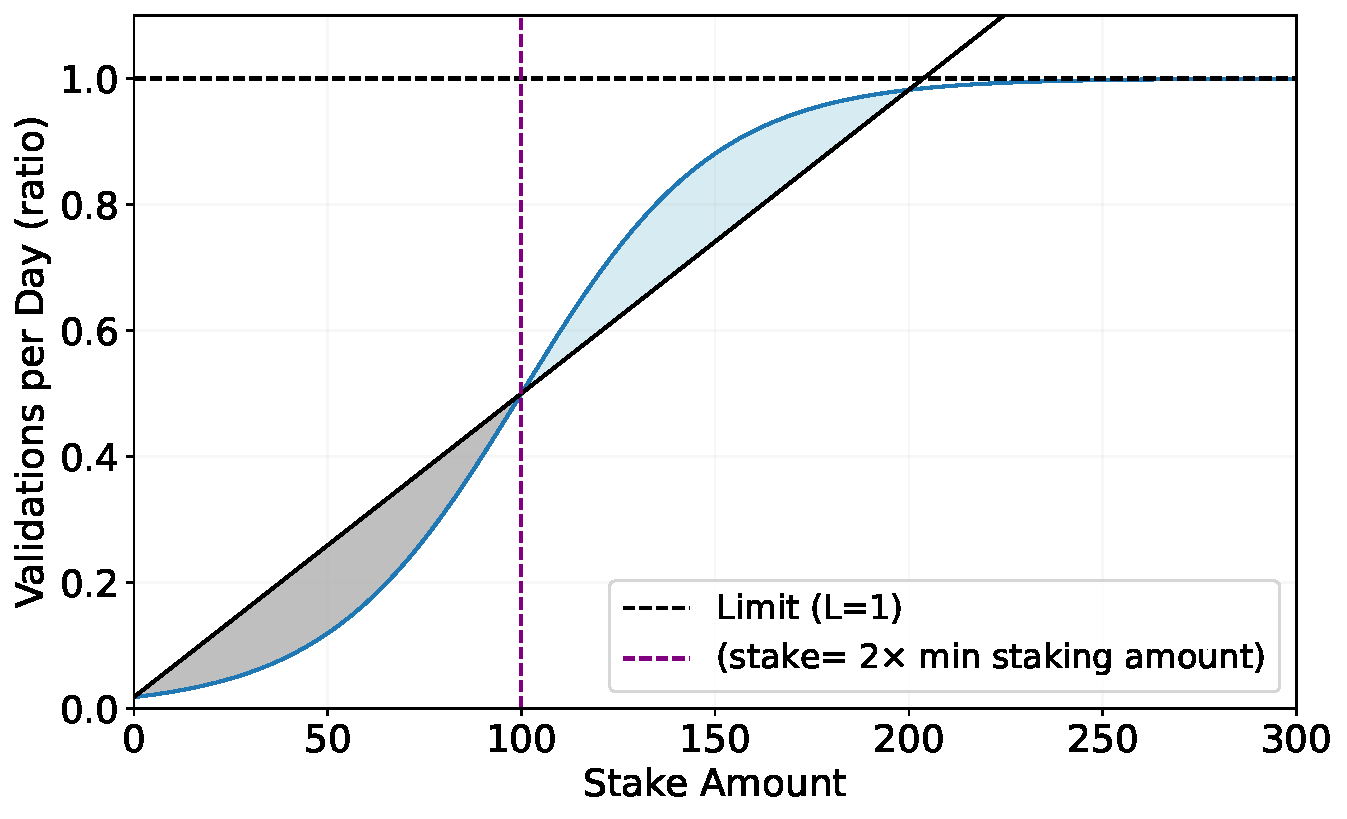
\includegraphics[width=\columnwidth]{figures/test_rate_limiting.pdf}
\caption{Example: rate limiting for validation frequency.}
\label{fig:test_rate_limiting}
\end{figure}

\subsection{Training in \SNT}

% \todo{@Ray, Can you please present the workflow of Single Node Training in FLock in more detail, including its training and validation?}

% \begin{table*}[t]
% \centering
% \renewcommand\arraystretch{2}
% \resizebox{2\columnwidth}{!}{%
% \begin{tabular}{lccccccccc}
% \toprule
% & \multirow{3}{*}{Total} & \multicolumn{4}{c}{\textbf{Rewards for Training Nodes}} & \multicolumn{4}{c}{\textbf{Rewards for Validators}} \\
% \cmidrule(lr){3-6} \cmidrule(lr){7-10}
% & & \multicolumn{2}{c}{Reward A} & \multicolumn{2}{c}{Reward B} & \multicolumn{2}{c}{Reward A} & \multicolumn{2}{c}{Reward B} \\
% \cmidrule(lr){3-4} \cmidrule(lr){5-6} \cmidrule(lr){7-8} \cmidrule(lr){9-10}
% & & \cellcolor{lightbrown}Node 1 & \cellcolor{lightgray}Node 2 & \cellcolor{lightbrown}Node 1 & \cellcolor{lightgray}Node 2 & \cellcolor{lightbrown}Validator 1 & \cellcolor{lightgray}Validator 2 & \cellcolor{lightbrown}Validator 1 & \cellcolor{lightgray}Validator 2 \\
% \midrule
% Day 1 & 200 & \cellcolor{lightbrown}$20 \times 0.7 \times 0.5 = 7$ & \cellcolor{lightgray}$20 \times 0.7 \times 0.5 = 7$ & \cellcolor{lightbrown}$180 \times 0.7 \times 0.5 = 63$ & \cellcolor{lightgray}$180 \times 0.7 \times 0.5 = 63$ & \cellcolor{lightbrown}$20 \times 0.3 \times 0.5 = 3$ & \cellcolor{lightgray}$20 \times 0.3 \times 0.5 = 3$ & \cellcolor{lightbrown}$180 \times 0.3 \times 0.5 = 27$ & \cellcolor{lightgray}$180 \times 0.3 \times 0.5 = 27$ \\
% Day 2 & 200 & \cellcolor{lightbrown}$20 \times 0.7 \times 0.5 = 7$ & \cellcolor{lightgray}$20 \times 0.7 \times 0.5 = 7$ & \cellcolor{lightbrown}$180 \times 0.7 \times 0.5 = 63$ & \cellcolor{lightgray}$180 \times 0.7 \times 0.5 = 63$ & \cellcolor{lightbrown}$20 \times 0.3 \times 0.5 = 3$ & \cellcolor{lightgray}$20 \times 0.3 \times 0.5 = 3$ & \cellcolor{lightbrown}$180 \times 0.3 \times 0.5 = 27$ & \cellcolor{lightgray}$180 \times 0.3 \times 0.5 = 27$ \\
% Day 3 & 200 & \cellcolor{lightbrown}$20 \times 0.7 \times 0.55 = 7.7$ & \cellcolor{lightgray}$20 \times 0.7 \times 0.45 = 6.3$ & \cellcolor{lightbrown}$180 \times 0.7 \times 0.55 = 69.3$ & \cellcolor{lightgray}$180 \times 0.7 \times 0.45 = 56.7$ & \cellcolor{lightbrown}$20 \times 0.3 \times 0.55 = 3.3$ & \cellcolor{lightgray}$20 \times 0.3 \times 0.45 = 2.7$ & \cellcolor{lightbrown}$180 \times 0.3 \times 0.55 = 29.7$ & \cellcolor{lightgray}$180 \times 0.3 \times 0.45 = 24.3$ \\
% Day 4 & 200 & \cellcolor{lightbrown}$20 \times 0.7 \times 0.55 = 7.7$ & \cellcolor{lightgray}$20 \times 0.7 \times 0.45 = 6.3$ & \cellcolor{lightbrown}$180 \times 0.7 \times 0.55 = 69.3$ & \cellcolor{lightgray}$180 \times 0.7 \times 0.45 = 56.7$ & \cellcolor{lightbrown}$20 \times 0.3 \times 0.55 = 3.3$ & \cellcolor{lightgray}$20 \times 0.3 \times 0.45 = 2.7$ & \cellcolor{lightbrown}$180 \times 0.3 \times 0.55 = 29.7$ & \cellcolor{lightgray}$180 \times 0.3 \times 0.45 = 24.3$ \\
% Day 5 & 333.33 & \cellcolor{lightbrown}$33.33 \times 0.7 \times 0.6 = 14$ & \cellcolor{lightgray}$33.33 \times 0.7 \times 0.4 = 9.33$ & \cellcolor{lightbrown}$300 \times 0.7 \times 0.5 = 105$ & \cellcolor{lightgray}$300 \times 0.7 \times 0.5 = 105$ & \cellcolor{lightbrown}$33.33 \times 0.3 \times 0.6 = 6$ & \cellcolor{lightgray}$33.33 \times 0.3 \times 0.4 = 4$ & \cellcolor{lightbrown}$300 \times 0.3 \times 0.5 = 45$ & \cellcolor{lightgray}$300 \times 0.3 \times 0.5 = 45$ \\
% \bottomrule
% \end{tabular}
% }
% \caption{Example: Reward distribution among the participants in task 1 over five days.}
% \label{tab:rewards_distribution-table2}
% \end{table*}


% We consider the dataset held by the training node, \(\mathcal{D}_{\text{local}}\), which contains locally sourced data samples. Datasets contributed by external contributors are represented as \(\mathcal{D}_{\text{contrib}}^i\), where \(i\) indexes each distinct contributor. The comprehensive dataset, denoted as \(\mathcal{D}\), integrates both local and external contributions, formulated as:
% \begin{equation*}
%     \mathcal{D} = \mathcal{D}_{\text{local}} \cup \left( \bigcup_{i=1}^{n} \mathcal{D}_{\text{contrib}}^i \right) 
% \end{equation*}
% comprising feature set \(X\) and label set \(Y\), with each sample \(x_i \in X\) corresponding to a label \(y_i \in Y\). We define a predictive model \(f\), aiming to learn patterns within \(\mathcal{D}\) such that \(f(x_i) \approx y_i\).

We consider the dataset held by the training node, \(\mathcal{D}_{\text{local}}\), which contains locally sourced data samples, comprising feature set \(X\) and label set \(Y\), with each sample \(x_i \in X\) corresponding to a label \(y_i \in Y\). We define a predictive model \(f\), aiming to learn patterns within \(\mathcal{D}\) such that \(f(x_i) \approx y_i\).

To quantify the prediction metric, accuracy as an example, the task trainer will introduce a loss function \(L(f(x_i), y_i)\), assessing the discrepancy between predictions \(f(x_i)\) and actual labels \(y_i\). A generic expression for this function is:
\begin{equation*}
L = \frac{1}{N} \sum_{i=1}^{N} l(f(x_i), y_i) 
\end{equation*}
where \(N\) denotes the total sample count, and \(l\) signifies a problem-specific loss function, e.g., mean squared error or cross-entropy loss.

The optimisation goal is to adjust the model parameters \(\theta\) to minimise \(L\), typically through algorithms such as  gradient descent:
\begin{equation*}
\theta_{\text{new}} = \theta_{\text{old}} - \eta \nabla_\theta L
\end{equation*}
where \(\eta\) represents the learning rate, and \(\nabla_\theta L\) the gradient of \(L\) with respect to \(\theta\). Utilising the aggregated dataset \(\mathcal{D}\), parameter \(\theta\) is iteratively updated to reduce \(L\), consequently improving the model's predictive accuracy. This optimisation process is conducted over a predefined number of epochs \(E\), each epoch consisting of a complete pass through the entire dataset \(\mathcal{D}\).








\subsection{Validation in \SNT}
% \todo{@Ray: can you please also finish this part of \SNT validation?}

Consider a selected group of validators, denoted as $V_j \in V$, each equipped with the evaluation dataset $\mathcal{D}_{\text{eval}}$ from the task creator. This dataset consists of pairs $(x_i, y_i)$, where $x_i$ represents the features of the $i$-th sample, and $y_i$ is the corresponding true label. 

The model, trained by designated training nodes, is denoted as $\theta^{task}_p$. The primary objective of $\theta^{task}_p$ is to predict the label $\hat{y}_i$ for each feature vector $x_i$ contained within $\mathcal{D}_{\text{eval}}$. 

To assess the performance of $\theta^{task}_p$ on $\mathcal{D}_{\text{eval}}$, we use an general evaluation metric denoted by $eval$. Here, we exemplify with accuracy, which is calculated as follows:

\begin{equation*}
eval(\theta^{task}_p, \mathcal{D}_{\text{eval}}) = \frac{1}{|\mathcal{D}_{\text{eval}}|} \sum_{(x_i, y_i) \in \mathcal{D}_{\text{eval}}} \mathbf{1}(\hat{y}_i = y_i)
\end{equation*}

Here, $\mathbf{1}$ represents the indicator function that returns 1 if the predicted label $\hat{y}_i$ matches the true label $y_i$, and 0 otherwise. The function $|\mathcal{D}_{\text{eval}}|$ denotes the total number of samples within the evaluation dataset.

Each predicted label $\hat{y}_i$ from the model $\theta^{task}_p$ is compared against its corresponding true label $y_i$ within the dataset $\mathcal{D}_{\text{eval}}$. The calculated metric result (accuracy here) serves as a quantifiable measure of $\theta^{task}_p$'s effectiveness at label prediction across the evaluation dataset. 


% Model Evaluation
% Once the model is trained, evaluate its performance using a set of independent test data \(\mathcal{D}_{\text{test}}\). The performance metrics (such as accuracy, recall, F1 score, etc.) depend on the specific problem.




\subsection{Reward for Training Nodes in \SNT}\label{sec: reward-for-training-nodes}







% \begin{itemize}
%     \item Given a task, consider the case that there are $n$ training nodes $(O_1, ..., O_n)$, and $m$ validators $(V_1, …, V_m)$ with stakes $(s_1, ..., s_m)$.
%     \item Each validator $V_j (1\le j\le m)$ will evaluate the $n$ models generated by the $n$ training nodes, and output the score vector $\vec{r_j} = (r_{j1}, ..., r_{jn})$ .
% \end{itemize}
% The final score is calculated through weighted aggregation:

%        $$\vec{r} = \left(\frac{\sum_j{r_{j1}\cdot s_j}}{\sum_j{s_j}}, ..., \frac{\sum_j{r_{jn}\cdot s_j}}{\sum_j{s_j}}\right)$$

% If the total reward for training nodes is $R_O$, then for a training node $O_i$, their reward is proportional to the corresponding (normalised) aggregated score

%       $$R_O \cdot \mathsf{Normalize}(\frac{\sum_j{r_{ji}\cdot s_j}}{\sum_j{s_j}})$$





We assume there are $n$ submissions $(O_1, \ldots, O_n)$ from $n$ training nodes, and $m$ validators $(V_1, \ldots, V_m)$, each with stakes $(s_1, \ldots, s_m)$. The stakes represent the validators' commitment and trust in the process, influencing the weight of their evaluations in the aggregated score.


\begin{itemize}

    \item Each validator $V_j (1\leq j\leq m)$ evaluates the $n$ models submitted by the training nodes, producing a score vector $\vec{r}_j = (r_{j1}, \ldots, r_{jn})$. These scores reflect the perceived accuracy, reliability, or performance of each model according to predefined criteria. The outlier scores proposed by malicious validators will be ignored by honest validators  before taking into amount in the following steps.
    
    \item The final score for each model from the training nodes is determined through a weighted aggregation:
    \[
    \vec{r} = \left(\frac{\sum_{j}{r_{j1}\cdot s_j}}{\sum_{j}{s_j}}, \ldots, \frac{\sum_{j}{r_{jn}\cdot s_j}}{\sum_{j}{s_j}}\right)
    \]
    This means that the evaluations of validators with higher stakes have a larger impact on the final outcome.
    
    \item We then compute the following geometry series:
    \[
    g_k =  \frac{1 - q}{1 - q^m} \cdot q^{k-1}
    \]
    
in which $k$ denotes a given training node's rank amongst its peers in the same task, whereas $q$ represents the common ratio of the geometric series and $m$ is the number of training nodes in a given task.

\item We finally compute the the reward allocated for the training nodes, which is based on the quality of their submission and their stake:

$$f_i(g_i, t_i) = \frac{e^{\lambda_t g_{i}} \cdot t_i^{\alpha_t}}{\sum_{k=1}^{n} e^{\lambda_t g_{k}} \cdot t_k^{\alpha_t}}
$$
where $\lambda_t$ and $\alpha_t$ are two system parameters, and $t_i$ the stake amount of node $i$.

    % \item Security and integrity of the evaluation process are paramount. Validators are incentivised to participate honestly through mechanisms such as slashing, where those who behave maliciously or negligently have their stakes reduced.
    % \item The system should also be safeguarded against collusion among validators or attempts to manipulate the evaluation process. Techniques such as advanced cryptography, reputation systems, and random validator selection can enhance trust and decentralisation in the evaluation framework.
\end{itemize}


\begin{table*}[t]
\centering
\renewcommand\arraystretch{1.75}
\resizebox{2\columnwidth}{!}{%
\begin{tabular}{lccccccccc}
\toprule
& \multirow{4}{*}{Total} & \multicolumn{6}{c}{\textbf{Rewards for Training Nodes}} & \multicolumn{2}{c}{\textbf{Rewards for Validators}} \\
\cmidrule(lr){3-8} \cmidrule(lr){9-10}
& & \multicolumn{3}{c}{Reward A} & \multicolumn{3}{c}{Reward B} & \cellcolor{lightbrown}Reward & \cellcolor{lightgray}Reward \\
\cmidrule(lr){3-5} \cmidrule(lr){6-8}
& & \cellcolor{lightbrown}Node 1 & \cellcolor{lightgray}Node 2 & \cellcolor{lightblue}Node 3 & \cellcolor{lightbrown}Node 1 & \cellcolor{lightgray}Node 2 & \cellcolor{lightblue}Node 3 & \cellcolor{lightbrown}Validator 1 & \cellcolor{lightgray}Validator 2 \\
\midrule
Day 1 & 200 & \cellcolor{lightbrown}$20 \times 0.5 \times 0.39 = 3.9$ & \cellcolor{lightgray}$20 \times 0.5 \times 0.33 = 3.3$ & \cellcolor{lightblue}$20 \times 0.5 \times 0.28 = 2.8$ & \cellcolor{lightbrown}$180 \times 0.5 \times 0.39 = 35.1$ & \cellcolor{lightgray}$180 \times 0.5 \times 0.33 = 29.7$ & \cellcolor{lightblue}$180 \times 0.5 \times 0.28 = 25.2$ & \cellcolor{lightbrown}$100 \times 0.4 = 40$ & \cellcolor{lightgray}$100 \times 0.6 = 60$ \\
Day 2 & 200 & \cellcolor{lightbrown}$20 \times 0.5 \times 0.39 = 3.9$ & \cellcolor{lightgray}$20 \times 0.5 \times 0.33 = 3.3$ & \cellcolor{lightblue}$20 \times 0.5 \times 0.28 = 2.8$ & \cellcolor{lightbrown}$180 \times 0.5 \times 0.39 = 35.1$ & \cellcolor{lightgray}$180 \times 0.5 \times 0.33 = 29.7$ & \cellcolor{lightblue}$180 \times 0.5 \times 0.28 = 25.2$ & \cellcolor{lightbrown}$100 \times 0.4 = 40$ & \cellcolor{lightgray}$100 \times 0.6 = 60$ \\
Day 3 & 200 & \cellcolor{lightbrown}$20 \times 0.5 \times 0.39 = 3.9$ & \cellcolor{lightgray}$20 \times 0.5 \times 0.33 = 3.3$ & \cellcolor{lightblue}$20 \times 0.5 \times 0.28 = 2.8$ & \cellcolor{lightbrown}$180 \times 0.5 \times 0.39 = 35.1$ & \cellcolor{lightgray}$180 \times 0.5 \times 0.33 = 29.7$ & \cellcolor{lightblue}$180 \times 0.5 \times 0.28 = 25.2$ & \cellcolor{lightbrown}$100 \times 0.45 = 45$ & \cellcolor{lightgray}$100 \times 0.55 = 55$ \\
Day 4 & 200 & \cellcolor{lightbrown}$20 \times 0.5 \times 0.39 = 3.9$ & \cellcolor{lightgray}$20 \times 0.5 \times 0.33 = 3.3$ & \cellcolor{lightblue}$20 \times 0.5 \times 0.28 = 2.8$ & \cellcolor{lightbrown}$180 \times 0.5 \times 0.39 = 35.1$ & \cellcolor{lightgray}$180 \times 0.5 \times 0.33 = 29.7$ & \cellcolor{lightblue}$180 \times 0.5 \times 0.28 = 25.2$ & \cellcolor{lightbrown}$100 \times 0.45 = 45$ & \cellcolor{lightgray}$100 \times 0.55 = 55$ \\
Day 5 & 200 & \cellcolor{lightbrown}$20 \times 0.5 \times 0.39 = 3.9$ & \cellcolor{lightgray}$20 \times 0.5 \times 0.33 = 3.3$ & \cellcolor{lightblue}$20 \times 0.5 \times 0.28 = 2.8$ & \cellcolor{lightbrown}$180 \times 0.5 \times 0.39 = 35.1$ & \cellcolor{lightgray}$180 \times 0.5 \times 0.33 = 29.7$ & \cellcolor{lightblue}$180 \times 0.5 \times 0.28 = 25.2$ & \cellcolor{lightbrown}$100 \times 0.5 = 50$ & \cellcolor{lightgray}$100 \times 0.5 = 50$ \\
\bottomrule
\end{tabular}
}
\caption{Example: Reward distribution among the participants in one task over five days.}
\label{tab:rewards_distribution-table2}
\end{table*}




\subsection{Reward for Validators in \SNT}\label{sec: reward-for-validators}

For each validator $V_j$, we compute the distances between their score and the final aggregated score:

\begin{equation*}
    \begin{aligned}
         \vec{\Delta_j} &= \left(\Delta_{j1}, ..., \Delta_{jn}\right)\\
         &= \left(\left|{\frac{\sum_j{r_{j1}\cdot s_j}}{\sum_j{s_j}}}-r_{j1}\right|, ..., \left|\frac{\sum_j{r_{jn}\cdot s_j}}{\sum_j{s_j}} - r_{jn}\right|\right) 
    \end{aligned}
\end{equation*}
We define a distribution function $f_i$, which satisfies: 
 
\[
\left\{
\begin{array}{l}
 f_i(\Delta_{1i}, s_1) + \ldots + f_i(\Delta_{mi}, s_m) = 1, \\
 f_i \text{ decreases over the distance } \Delta_{ji}, \\
 f_i \text{ increases over the stake amount } s_j.
\end{array}
\right.
\]

% $f_i(\Delta_{1i}, s_1) + ... + f_i(\Delta_{mi}, s_m) = 1$ and $f_i$ decreases over the distance $\Delta_{ji}$, but $f_i$ increases over the stake amount $s_j$.

% - We can use a modified version of \href{https://en.wikipedia.org/wiki/Softmax_function}{Softmax Function}:
%     $$f_i(\Delta_{ji}, s_j) = \frac{e^{-\lambda \Delta_{ji}} \cdot s_j^{\alpha}}{\sum_{k=1}^{m} e^{-\lambda \Delta_{ki}} \cdot s_k^{\alpha}}$$

To fulfill the three criteria, we can employ a modified version of the Softmax Function:
    $$f_i(\Delta_{ji}, s_j) = \frac{e^{-\lambda_v \Delta_{ji}} \cdot s_j^{\alpha_v}}{\sum_{k=1}^{m} e^{-\lambda_v \Delta_{ki}} \cdot s_k^{\alpha_v}}$$




% Other options of $f$:

% $$f_i(\Delta_{ji}, s_j) = \frac{\frac{1}{1 + \lambda \Delta_{ji}} \cdot s_j}{\sum_{k=1}^{m} \frac{1}{1 + \lambda \Delta_{ki}} \cdot s_k}$$

% $$f_i(\Delta_{ji}, s_j) = \frac{(1 - \lambda \Delta_{ji}) \cdot s_j}{\sum_{k=1}^{m} (1 - \lambda \Delta_{ki}) \cdot s_k}$$ (in this case, we should normalise $\Delta_{ji}$)





The parameters $\lambda$ and $\alpha$ play  crucial roles:





\begin{itemize}
    \item {$\lambda_v$}

\begin{itemize}
    \item Purpose: Controls the sensitivity of the function to the distance $\Delta_{ji}$. This distance measures the discrepancy between a validator's score and the aggregated score.
    \item Effect: A higher $\lambda_v$ increases the function's sensitivity to score accuracy, emphasising the importance of precise evaluations.
    
    \item Selection Criteria: The choice of $\lambda_v$ balances the need to penalise inaccuracies against the goal of rewarding nearly accurate evaluations.
\end{itemize}

\item {$\alpha_v$}
\begin{itemize}
    \item Purpose: Determines the influence of the stake amount $s_j$ on the reward distribution, thereby adjusting the weight given to validators' financial contributions.
    
    \item Effect:  Allows for balancing between the importance of validators' financial commitment and their performance accuracy. A higher $\alpha_v$ gives more weight to the stake amount in the reward calculation.
    
    \item Selection Criteria: Reflects the system's philosophy regarding the stake's importance relative to score accuracy. An $\alpha_v$ of 0 means stake amounts are ignored, while a higher value increases their impact.
\end{itemize}
\end{itemize}


If the validator finishes multiple (i.e., $N$) validation tasks, then it reward ratio is:

$$\sum_{i = 1}^{N}{f_i(\Delta_{ji}, s_j)}$$


If a validator’s stake in the task is $s_v$, and $s_j$ is its accumulative stake by considering the total delegation amount $S_d$ on this validator, i.e., $s_j = s_v + S_d$, the actual reward ratio for this valdiator is:

$$\left(\sum_i{f_i(\Delta_{ji}, s_j)}\right) \cdot \left(\sigma + (1-\sigma) \cdot \frac{s_v}{s_v+S_d}\right)$$

where $\sigma$ is a system parameter.


\subsection{Delegate Staking}
Delegators may entrust their tokens to participants of their choosing to receive a passive investment income stream. The receivers can thus amplify their stake, influence, voting power, and rewards. These rewards are shared with the delegators, furthering cooperation. This extends participation to users who have tokens but lack the technical expertise to perform AI model training or validation.

Specifically, reward for the delegator depends on:
\begin{itemize}
    \item The quality of the validators selected, as measured by the score variance of the delegated validator.
    \item The amount of stake delegator has delegated.
\end{itemize}

Formally, reward for delegator can be calculated as:

    $$\left(\sum_i{f_i(\Delta_{ji}, s_j)}\right) \cdot \sigma \cdot \frac{s_d}{s_v+S_d}$$
in which $\sum_i{f_i(\Delta_{ji}, s_j)}$ is the Softmax function for validator mentioned above, whereas $s_d$ refers to the stake amount from a given delegator and $s_v$ is the stake amount of the validator the delegator delegated to.

In the future, FLock delegate staking has the option to be integrated with existing restaking platforms to attract users from a border blockchain community.

\begin{figure*}[t]
\centering
\includegraphics[width=2\columnwidth]{figures/FLock_FL_part.pdf}
\caption{Overview of the workflow of a FLock FL task, adopted from our previous work~\cite{dong2023defending}. 
During each round, FL clients are randomly selected to act as proposers or voters. Their staked amount can be either rewarded or slashed based on the outcome of the majority voting results. Malicious clients will ultimately be removed from the FL system.}
\label{fig:FLock_FL_part}
\end{figure*}



\subsection{Various Validation Sets} To mitigate the lookup attacks from malicious training nodes, FLock validators adopt diverse validation datasets. Specifically, for a \SNT task spanning $x$ days, the validation dataset used during the initial $x-1$ days differs from that of the final day. These distinct validation datasets are associated with two types of rewards: \textbf{Reward A} for the initial period and \textbf{Reward B} for the final day. This strategic approach enhances security by varying the data against which training nodes are validated, thereby complicating any potential malicious attempts to exploit predictable validation scenarios.


\begin{itemize}
    \item For each \SNT within the ecosystem, the rewards mechanism for training nodes is thoughtfully designed to comprise two distinct parts: \textbf{Reward A} and \textbf{Reward B}.  

    \begin{itemize}
        % \item  \textbf{Reward A }represents the portion of rewards that is emitted on a daily basis. This continuous emission serves as an immediate incentive for participants, rewarding ongoing engagement and contribution to the \SNT tasks. The daily emission of Reward A ensures that participants receive consistent feedback and gratification for their contributions.
        \item \textbf{Reward A} provides a daily contingent reinforcement schedule, incentivizing participant engagement with \SNT tasks through immediate gratification. This continuous reward mechanism fosters sustained participation by providing consistent feedback and reinforcing contributions.
        \item \textbf{Reward B}, implements vesting, releasing tokens upon successful task completion within a predetermined lifespan. This incentivizes participants to both engage in tasks and ensure their timely and efficient completion. Vesting also functions as a quality control mechanism, promoting focused contributions aligned with project deadlines.
        % on the other hand, introduces a vesting component to the rewards structure. This portion of the reward is reserved and only emitted upon the completion of a task, provided that the task does not exceed its maximum lifecycle. The inclusion of Reward B as a vested reward serves multiple purposes. It incentivises participants to not only engage with tasks but to see them through to completion, ensuring that tasks are not abandoned prematurely. Furthermore, by withholding a portion of the rewards until task completion and ensuring they are only distributed if the task is completed within its designated lifecycle, Reward B acts as a quality control mechanism, encouraging efficient and timely contribution towards task goals.
    \end{itemize}
   
            \begin{itemize}
            \item Reward A of the \SNT task is: 
            $$R^{AI, A}_i = \delta \cdot R^{AI}_i$$ 
            
% $$R^{AI, A}_i = \delta \cdot C \cdot \frac{S_i}{\sum_{k=1}^{M}{S_k} + \tau \cdot\sum_{j=1}^{N}{F_j \cdot P_j}}$$ 

        \item Reward B of the \SNT task is:
        $$R^{AI, B}_i = (1-\delta) \cdot R^{AI}_i$$

        \end{itemize}
        $\delta$ is a configurable system parameter.



\end{itemize}

\subsection{Example} 

We consider the rewards for the participants in task 1.

We assume that:
\begin{itemize}
    \item Distribution among the participants with a task is: task creator ($0\%$), training nodes ($50\%$), and validators ($50\%$);
    \item There are three training nodes: Node 1, Node 2 and Node 3, meaning $m$, the number of training nodes in a given task, is 3;
    \item Nodes 1, 2 and 3 rank first, second and third respectively, and assume their respective rankings remain the same every day and they have the same amount of stake;
    \item $q$, which is the order of geometry series, is 0.85;
    \item There are two validators: Validator 1 and Validator 2;
    \end{itemize}
 Thus, their reward distribution during the five days are:
    \begin{itemize}
        \item Day 1: (Node 1: $0.39$, Node 2: $0.33$, Node 3: 0.28), (Validator 1: $0.4$, Validator 2: $0.6$);
        \item Day 2: (Node 1: $0.39$, Node 2: $0.33$, Node 3: 0.28), (Validator 1: $0.4$, Validator 2: $0.6$);
        \item Day 3: (Node 1: $0.39$, Node 2: $0.33$, Node 3: 0.28), (Validator 1: $0.45$, Validator 2: $0.55$);
        \item Day 4: (Node 1: $0.39$, Node 2: $0.33$, Node 3: 0.28), (Validator 1: $0.45$, Validator 2: $0.55$);
        \item Day 5: (Node 1: $0.39$, Node 2: $0.33$, Node 3: 0.28), (Validator 1: $0.5$, Validator 2: $0.5$);
    \end{itemize}


The reward distribution among the participants in task 1 during the 5 days is shown in Table~\ref{tab:rewards_distribution-table2}.





\begin{figure*}[t]
\begin{mdframed}[backgroundcolor=gray!10, roundcorner=10pt]
\begin{algorithm}[H]
    \centering
    \begin{algorithmic}[1]
    \Statex 
    \Statex 
        \Statex $T$: Total number of global communication rounds
        \Statex $E$: Total number of local model update epochs
        \Statex $\theta_g$: Global model
        \Statex $\mathcal{D}_p^{train}$: local training dataset 
        \Statex $\mathcal{D}_p^{test}$: local test dataset 

    \Procedure{Init}{} 
        \State Download pre-trained model from AI Arena or initialise global model $\theta^t_g$
        \State Broadcast $\theta^t_g$ to all participants
    \EndProcedure
    
    \Procedure{Update}{$\theta^t_g$}
        \State Initialise local model $\theta^t_p$
        \State Update model parameters  $\theta^t_p \leftarrow \theta^t_g$
        \State $\theta^{t+1}_p \leftarrow \theta^{t}_p - \eta \nabla L(\theta^t_p ; b)$ \textcolor[HTML]{5E81B5}{\Comment{Local model update}}
        \State \Return $\theta^{t+1}_p$
    \EndProcedure

    \Procedure{Evaluate}{$\theta_t+1^P$}
        \State $\theta^{t+1}_g \leftarrow \sum_{p=1}^P \frac{n_p}{N} \theta_p^{t+1}$ \textcolor[HTML]{5E81B5}{\Comment{Model updates aggregation}}

        \State $\text{Res} \xleftarrow{\theta^{t+1}_g} \mathcal{D}_p^{test}$  \textcolor[HTML]{5E81B5}{\Comment{Evaluate aggregated model}}
        
        \State \Return $\text{Res}$
    \EndProcedure

    \Procedure{\textcolor[HTML]{EF6C63}{\textbf{Main}}}{}
        \State Random select initialisation leader $\rightarrow p_{lead}$
        \State $\rightarrow p_{lead}$ Do procedure \textbf{Init}
        \For{$t = 1 $ \textbf{to} $T$}
            \State Random assign roles for all participants
            \State Proposer does procedure \textbf{Update}
            \State Voter does procedure \textbf{Evaluate}
            \State $\mathsf{vote}_p^t \xleftarrow{\text{calculate}} \text{Res}^t_p$
            \State $\mathsf{aggVote}^t= \sum_{p = 1}^{ P_v}  \mathsf{vote}_p^t$ \textcolor[HTML]{5E81B5}{\Comment{Votes aggregation}}
            % \State $\theta^{t+1}_g \leftarrow$ Algorithm~\ref{algo:1}
            \State $\theta^{t+1}_g \leftarrow$ GlobalModelSelection($\mathsf{aggVote}^t$)
            \State Broadcast $\theta^{t+1}_g$
        \EndFor
    \EndProcedure
    
    \end{algorithmic}
    \caption{FLock Federated Training.}
    \label{algo:federated_learning}
\end{algorithm}
\end{mdframed}
\end{figure*}


\begin{figure*}[htbp]
\begin{mdframed}[backgroundcolor=gray!10, roundcorner=10pt]
\begin{algorithm}[H]
    \centering
    \begin{algorithmic}[1]
    \Statex 
    \Statex 
        \Statex $\mathcal{P}$: Set of participants at round $t$
        % \Statex ${totalStakedTokens}$: Accumulated proposers' staking tokens governed by smart contracts

        \Statex ${rewardPool}$: Total reward pool
        
        \Statex $\mathsf{Bal}_k$: Stake amount of participant $k$
    
        \Statex $s_p$: Slashed rate

        \Statex $participantsDistributionRate$: Ratio of participants in one round
        
        \Statex $\mathsf{TotalRounds}$: \rui{Total numbers of communication round}
        % \Statex $\mathsf{Num}_p$: Number of selected proposers per round

        % \Statex $\mathsf{Num}_v$: Number of selected voters per round
        
        \Statex $\mathsf{BalThreshold}_p$: minimum stake of participants


        \State ${pool}_p \leftarrow initialRewardPoolSize$
        % \For{$t = 0; t < \mathsf{TotalEpoch}$}
        \For{\rui{$t = 0; t < \mathsf{TotalRounds}$}}
        % \State ${pool}_p \leftarrow {pool}_p + mint_p$
        
        \State $\mathsf{Candidates} \leftarrow \{\}$
        
        \For {$k \in \mathcal{P} $}
        \If{$\mathsf{Bal}_k \geq \mathsf{BalThreshold}_p$}
        \State $\mathsf{Candidates} \leftarrow \mathsf{Candidates} \cup \{k\}$
        \EndIf
        \EndFor
        \State $\mathcal{P}_p^t, \mathcal{P}_v^t\leftarrow$ Randomly select proposers and voters from $\mathsf{Candidates}$ based on $participantsDistributionRate$


        \State $\mathsf{aggVote}^t \leftarrow$ Aggregated voting results from the voters $ \mathcal{P}_v^t$ at round $t$

 

        \State
        $roundRewardAmount \leftarrow \frac{{pool}_p}{\mathsf{TotalRounds} -t }$


               % \State $roundTotalStakedTokens$: compute the total stake amount of participants of this round
     
\State $roundTotalStakedTokensForGoodParticipants \leftarrow 0$

% \\ 
% \texttt{\color{gray}// Compute the participants that should be rewarded in this round}

\If {$\mathsf{aggVote}^t \geq 0$} \textcolor[HTML]{5E81B5}{\Comment{Compute the participants that should be rewarded in this round}}
        \For{$k \in \mathcal{P}_p^t$}
            \State $roundTotalStakedTokensForGoodParticipants ~+= \mathsf{Bal}_k$
        \EndFor
\EndIf
 \For{$k \in \mathcal{P}_v^t$}
        \If {$\mathsf{vote}_k^t \cdot \mathsf{aggVote}^t \geq 0$}
            \State  $roundTotalStakedTokensForGoodParticipants ~+= \mathsf{Bal}_k$
            \EndIf
        \EndFor
       
        
        
        % \\ \texttt{\color{gray}// Reward and Slash Proposers}
        
        \If {$\mathsf{aggVote}^t \geq 0$} \textcolor[HTML]{5E81B5}{\Comment{Reward and Slash Proposers}}
        

        \For{$k \in \mathcal{P}_p^t$}
            \State $\mathsf{Bal}_k \leftarrow \mathsf{Bal}_k + roundRewardAmount \cdot \frac{\mathsf{Bal}_k}{ roundTotalStakedTokensForGoodParticipants}$
            \State { ${pool}_p \leftarrow {pool}_p - roundRewardAmount \cdot \frac{\mathsf{Bal}_k}{ roundTotalStakedTokensForGoodParticipants}$}
        \EndFor
        
        \Else
        \For{$k \in \mathcal{P}_p^t$}
            \State $\mathsf{Bal}_k \leftarrow \mathsf{Bal}_k - \mathsf{Bal}_k \cdot s_p$
            \State ${pool}_p \leftarrow {pool}_p + \mathsf{Bal}_k \cdot s_p$
        \EndFor
        \EndIf
        % \\ \texttt{\color{gray}// Reward and Slash Voters}
        
        \For{$k \in \mathcal{P}_v^t$} \textcolor[HTML]{5E81B5}{\Comment{Reward and Slash Voters}}
        \If {$\mathsf{vote}_k^t \cdot \mathsf{aggVote}^t \geq 0$}
        % \\ \texttt{\color{gray}// The vote result aligns with the aggregated one}
            \State $\mathsf{Bal}_k \leftarrow \mathsf{Bal}_k + roundRewardAmount \cdot \frac{\mathsf{Bal}_k}{ roundTotalStakedTokensForGoodParticipants}$
            \State { ${pool}_p \leftarrow {pool}_p - roundRewardAmount \cdot \frac{\mathsf{Bal}_k}{ roundTotalStakedTokensForGoodParticipants}$}
            \Else
            \State $\mathsf{Bal}_k \leftarrow \mathsf{Bal}_k - \mathsf{Bal}_k \cdot s_p$
            \State ${pool}_p \leftarrow {pool}_p + \mathsf{Bal}_k \cdot s_p$
            \EndIf
        \EndFor
        
        \State $ t \leftarrow t + 1$
        \EndFor
    \end{algorithmic}
    \caption{Reward-and-slash design for FL clients.}
    \label{algo:all-fl-rewards}
\end{algorithm}
\end{mdframed}
\end{figure*}

% \subsection{Federated Learning}
\section{FLock Consensus in \FL}
Figure~\ref{fig:FLock_FL_part} depicts the workflow of a \FL task in FLock. As shown in our work in leveraging blockchain to defend against poisoning attacks in \FL~\cite{dong2023defending}, FLock adopts a distributed voting and a reward-and-slash mechanism to construct secure \FL systems.

% Assume there is an aggregator and $P$ participants in a \FL task, denoted as $\mathcal{P} = \{1, ..., P \}$.  Each participant needs to stake a predefined amount of coins to join the system.



\subsection{Task Creators}
Similar to task creation in \SNT, an \FL task creator must satisfy predefined criteria. Only \FL tasks verified by the FLock DAO will be eligible for rewards from the daily emissions. Otherwise, the \FL task creator must self-fund the reward pool using their own \FML.


% \subsubsection{VRF Selecion} For each round of the \FL task, a participant will be randomly selected as a training node/proposer or a validator/voter based on on-chain \VRF. A training node uploads their local model or gradient updates to the \FL aggregator. The aggregator will aggregate the local model or gradient updates from the training nodes. A validator will download the aggregated model updates and validate them to generate a score. For each participant, their local dataset can be randomly split into a training set and a test set, which will not be shared with other participants. Assume that for each round there are $P_T$ training nodes and $P_V$ validators. 

\subsection{Random Role Selection} 
Consider a \FL task involving $P$ participants, denoted as $\mathcal{P} = {1, \ldots, P}$. To participate in the training process, each participant needs to stake a specified quantity of coins. \rui{Upon formally joining the training task, each participant's local dataset $\mathcal{D}_p$ is randomly partitioned into a training set $\mathcal{D}_p^{train}$ and a test set $\mathcal{D}_p^{test}$, which will not be shared with other participants at any time. At the beginning of each round $t$ in the \FL task, participants are randomly assigned roles as either a proposer ($P_T$) or a voter ($P_V$) through an on-chain random function. Subsequently, a model initialised or pre-trained model downloaded from AI Arena by one of the proposers is chosen at random temporarily to serve as the pioneering global model. The selected model's weights or gradients are then distributed to all participants, ensuring a unified starting point for local models. Proposers are responsible for training their local models using their own data and subsequently sharing the updated model weights or gradients with all participants. Voters, on the other hand, aggregate these updates from proposers. They then proceed to validate the aggregated model updates, resulting in the generation of a validation score.
}





% \subsubsection{\FL Training} At the beginning of round $t$, the training nodes will first download the global model, $\theta^{t-1}$, which has been finalised in round $t-1$.
% \todo{@Ray, Can you please present the workflow of FL training in FLock in more detail?}
\subsection{\FL Training} At the start of round $t$, proposers initially download the global model, denoted as $\theta^{t-1}$, which was finalised in the previous round $(t-1)$. Using the local training dataset $\mathcal{D}_p^{train}$, proposers then proceed to update the model $\theta^{t-1}$ through $E$ epochs of local training. Then the updated model $\theta^{t}$ of the current round $t$ will be uploaded to the voters for evaluation.

% update equation here, similar with SNT




\subsection{\FL Aggregation}
% Upon the completion of task training during round $t$, the local models $\{\theta_p^{t}\}_{p=1}^{P_T}$ are collected and aggregated by the aggregator through a weighted mean as follows:
% \begin{equation*}
% \hat{\theta^t} = \sum_{p=1}^K \beta_p \cdot \theta_p^{t}
% \label{eq:WeightedAvg}
% \end{equation*}
% where the weight $\beta_p = \frac{n_p}{N}$. Here, $n_p = |\mathcal{D}_p|$ represents the count of local training data points within client $p$, and $N = \sum_{p=1}^{P_T} n_p$ denotes the aggregate count of training data points across all $P_T$ clients.

\rui{Upon the completion of task training during round $t$, the voter gathers the local models $\{\theta_p^{t}\}_{p=1}^{P_T}$ from proposers. These models are then aggregated into the latest global model using a weighted averaging approach, as described below:
\begin{equation*}
\hat{\theta^t} = \sum_{p=1}^{P_T} \beta_p \cdot \theta_p^{t}
\label{eq:WeightedAvg}
\end{equation*}
Here, the weight $\beta_p$ is defined as $\frac{n_p}{N}$, with $n_p = |\mathcal{D}_p^{train}|$ indicates the number of local training data samples for each proposer $p$, and $N = \sum_{p=1}^{P_T} n_p$ is the total number of training data samples across all proposers $P_T$. 
}



% \begin{figure}[t]
% \begin{mdframed}[backgroundcolor=gray!10, roundcorner=10pt]
% \begin{algorithm}[H]
%     \centering
%     \begin{algorithmic}[1]
%     \Statex 
%     \Statex 
%         \Statex $\mathcal{P}$: Set of participants at round $t$
%         \Statex ${pool}_p$: Accumulated proposers' staking tokens governed by smart contracts
        
%         \Statex $\mathsf{Bal}_k$: Balance of participant $k$
        
%         \Statex $r_p$: Rewarded tokens for proposing
%         \Statex $s_p$: Slashed tokens for proposing
%         \Statex $mint_p$: New created tokens per round for proposers
        
%         \Statex $\mathsf{TotalRounds}$: \rui{Total numbers of communication round}
%         \Statex $\mathsf{Num}_p$: Number of selected proposers per round
%         \Statex $\mathsf{BalThreshold}_p$: Balance threshold to select proposers


%         \State ${pool}_p \leftarrow 0$
%         % \For{$t = 0; t < \mathsf{TotalEpoch}$}
%         \For{\rui{$t = 0; t < \mathsf{TotalRounds}$}}
%         \State ${pool}_p \leftarrow {pool}_p + mint_p$
%         \State $\mathsf{Candidates} \leftarrow \{\}$
        
%         \For {$k \in \mathcal{P} $}
%         \If{$\mathsf{Bal}_k \geq \mathsf{BalThreshold}_p$}
%         \State $\mathsf{Candidates} \leftarrow \mathsf{Candidates} \cup \{k\}$
%         \EndIf
%         \EndFor
%         \State $\mathcal{P}_p^t \leftarrow$ Randomly select $\mathsf{Num}_p$ clients from $\mathsf{Candidates}$


%         \State $\mathsf{aggVote}^t \leftarrow$ Aggregated voting results from voters at round $t$
        
        
%         \If {$\mathsf{aggVote}^t \geq 0$} 
%         \For{$k \in \mathcal{P}_p^t$}
%             \State $\mathsf{Bal}_k \leftarrow \mathsf{Bal}_k + r_p$
%             \State ${pool}_p \leftarrow {pool}_p - r_p$
%         \EndFor
        
%         \Else
%         \For{$k \in \mathcal{P}_p^t$}
%             \State $\mathsf{Bal}_k \leftarrow \mathsf{Bal}_k - s_p$
%             \State ${pool}_p \leftarrow {pool}_p + s_p$
%         \EndFor
%         \EndIf
%         \State $ t \leftarrow t + 1$
%         \EndFor
%     \end{algorithmic}
%     \caption{Reward-and-slash design for FL proposers.}
%     \label{algo:1}
% \end{algorithm}
% \end{mdframed}
% \end{figure}






% \begin{figure}[t]
% \begin{mdframed}[backgroundcolor=gray!10, roundcorner=10pt]
% \begin{algorithm}[H]
%     \centering
%     \begin{algorithmic}[1]
%     \Statex 
%     \Statex 
%         \Statex $\mathcal{P}$: Set of participants at round $t$
%         \Statex ${pool}_v$: Accumulated voters' tokens governed by smart contracts
        
%         \Statex $\mathsf{Bal}_k$: Balance of participant $k$
        
%         \Statex $r_v$: Rewarded tokens for voting
%         \Statex $s_v$: Slashed tokens for voting
%         \Statex $mint_v$: New created tokens per round for voters
        
        
%         % \Statex $\mathsf{TotalEpoch}$: Total number of round
%         \Statex $\mathsf{TotalRounds}$: \rui{Total numbers of communication round}
%         \Statex $\mathsf{Num}_v$: Number of selected voters per round
%         \Statex $\mathsf{BalThreshold}_v$: Balance threshold to select voters


%         \State ${pool}_v \leftarrow 0$
%         % \For{$t = 0; t < \mathsf{TotalEpoch}$}
%         \For{\rui{$t = 0; t < \mathsf{TotalRounds}$}}
%         \State ${pool}_v \leftarrow {pool}_v + mint_v$
%         \State $\mathsf{Candidates} \leftarrow \{\}$
        
%         \For {$k \in \mathcal{P} $}
%         \If{$\mathsf{Bal}_k \geq \mathsf{BalThreshold}_v$}
%         \State $\mathsf{Candidates} \leftarrow \mathsf{Candidates} \cup \{k\}$
%         \EndIf
%         \EndFor
%         \State $\mathcal{P}_v^t \leftarrow$ Randomly select $\mathsf{Num}_v$ clients from $\mathsf{Candidates}$


%         \State $\mathsf{aggVote}^t \leftarrow$ Aggregated voting results from voters at round $t$


%         \For{$k \in \mathcal{P}_v^t$}
%         \If {$\mathsf{vote}_k^t \cdot \mathsf{aggVote}^t \geq 0$}
%         \\ \texttt{\color{gray}// The vote result aligns with the aggregated one}
%             \State $\mathsf{Bal}_k \leftarrow \mathsf{Bal}_k + r_v$
%             \State ${pool}_v \leftarrow {pool}_v - r_v$
%             \Else
%             \State $\mathsf{Bal}_k \leftarrow \mathsf{Bal}_k - s_v$
%             \State ${pool}_v \leftarrow {pool}_v + s_v$
%             \EndIf
%         \EndFor
%         \State $ t \leftarrow t + 1$
%         \EndFor
%     \end{algorithmic}
%     \caption{Reward-and-slash design for \FL voters.}
%     \label{algo:2}
% \end{algorithm}
% \end{mdframed}
% \end{figure}

% \begin{figure}[t]
% \centering
% 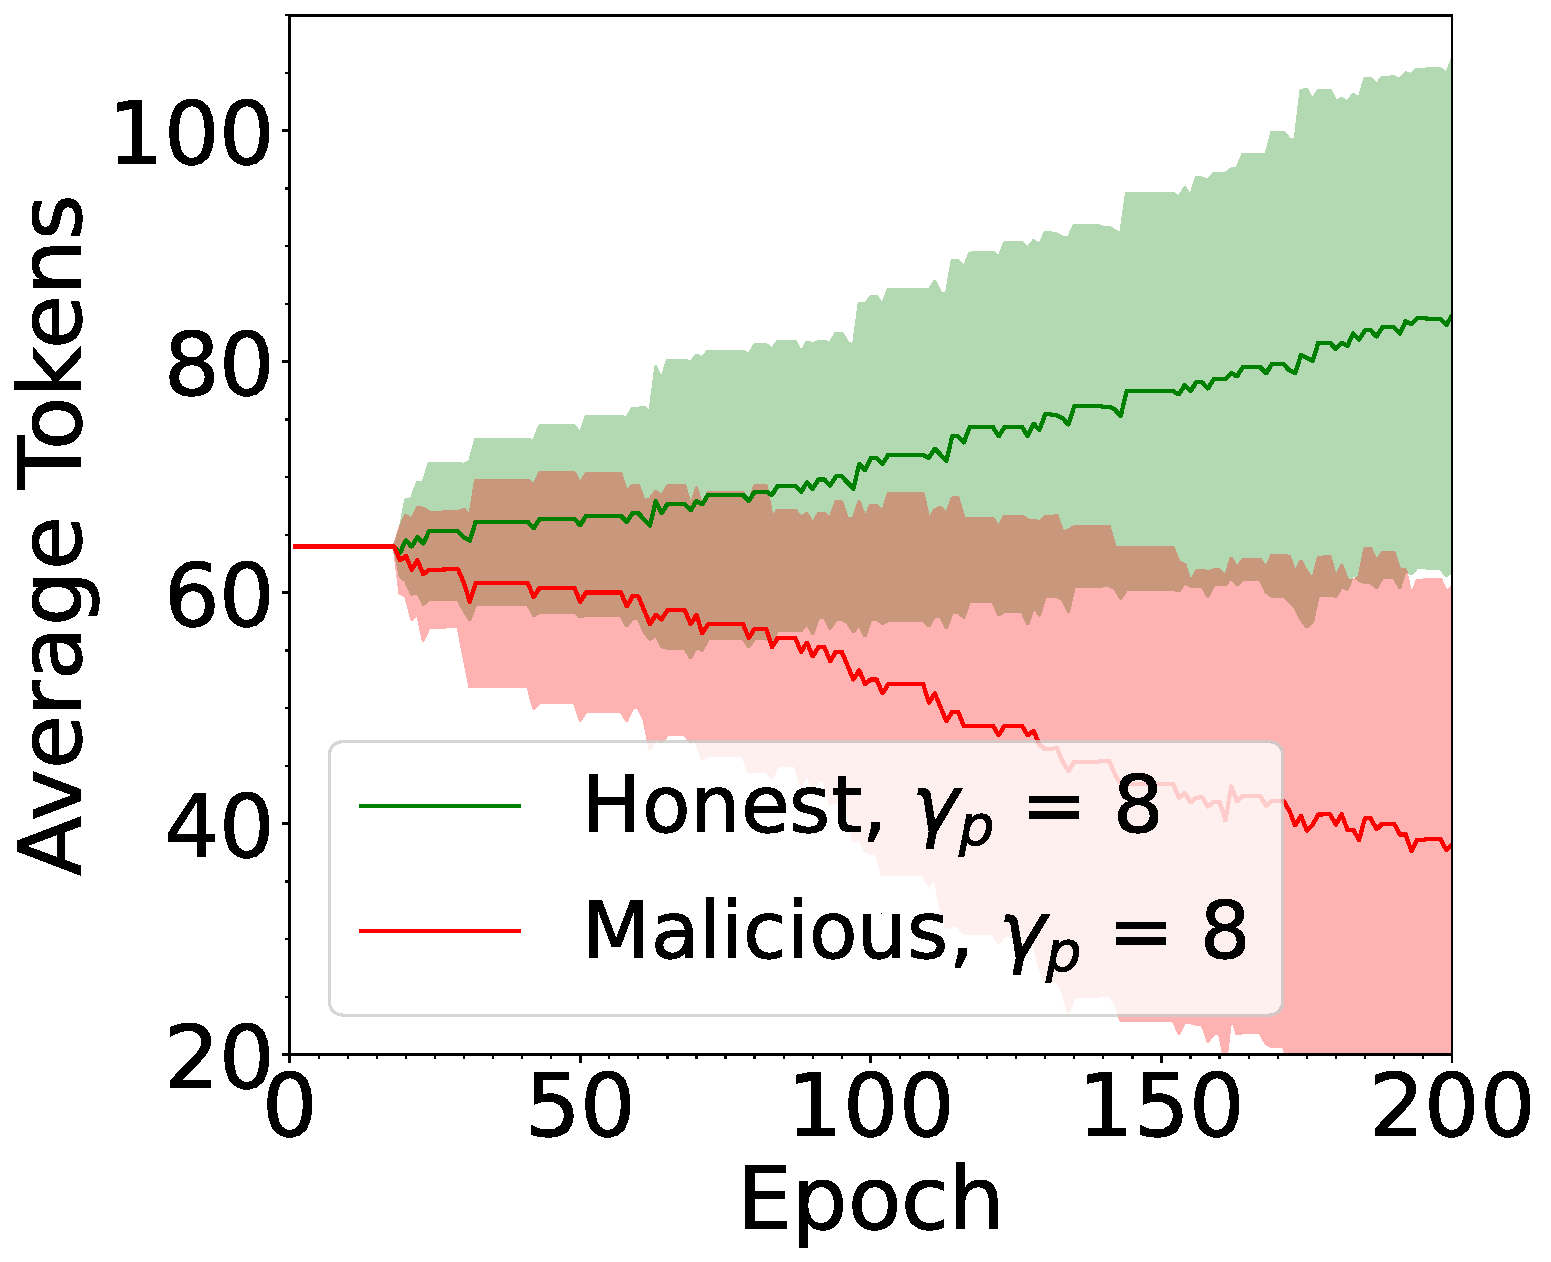
\includegraphics[width=\columnwidth]{figures/tokens_with_rate_0.4.pdf}
% \caption{Example of FL system with reward and slash mechanism, taken from~\cite{dong2023defending}. }
% \label{fig:tokens_with_rate_0.4}
% \end{figure}


\begin{figure*}[t]
\centering
\hfill
\subfigure[$\eta$ = 0.1.]{
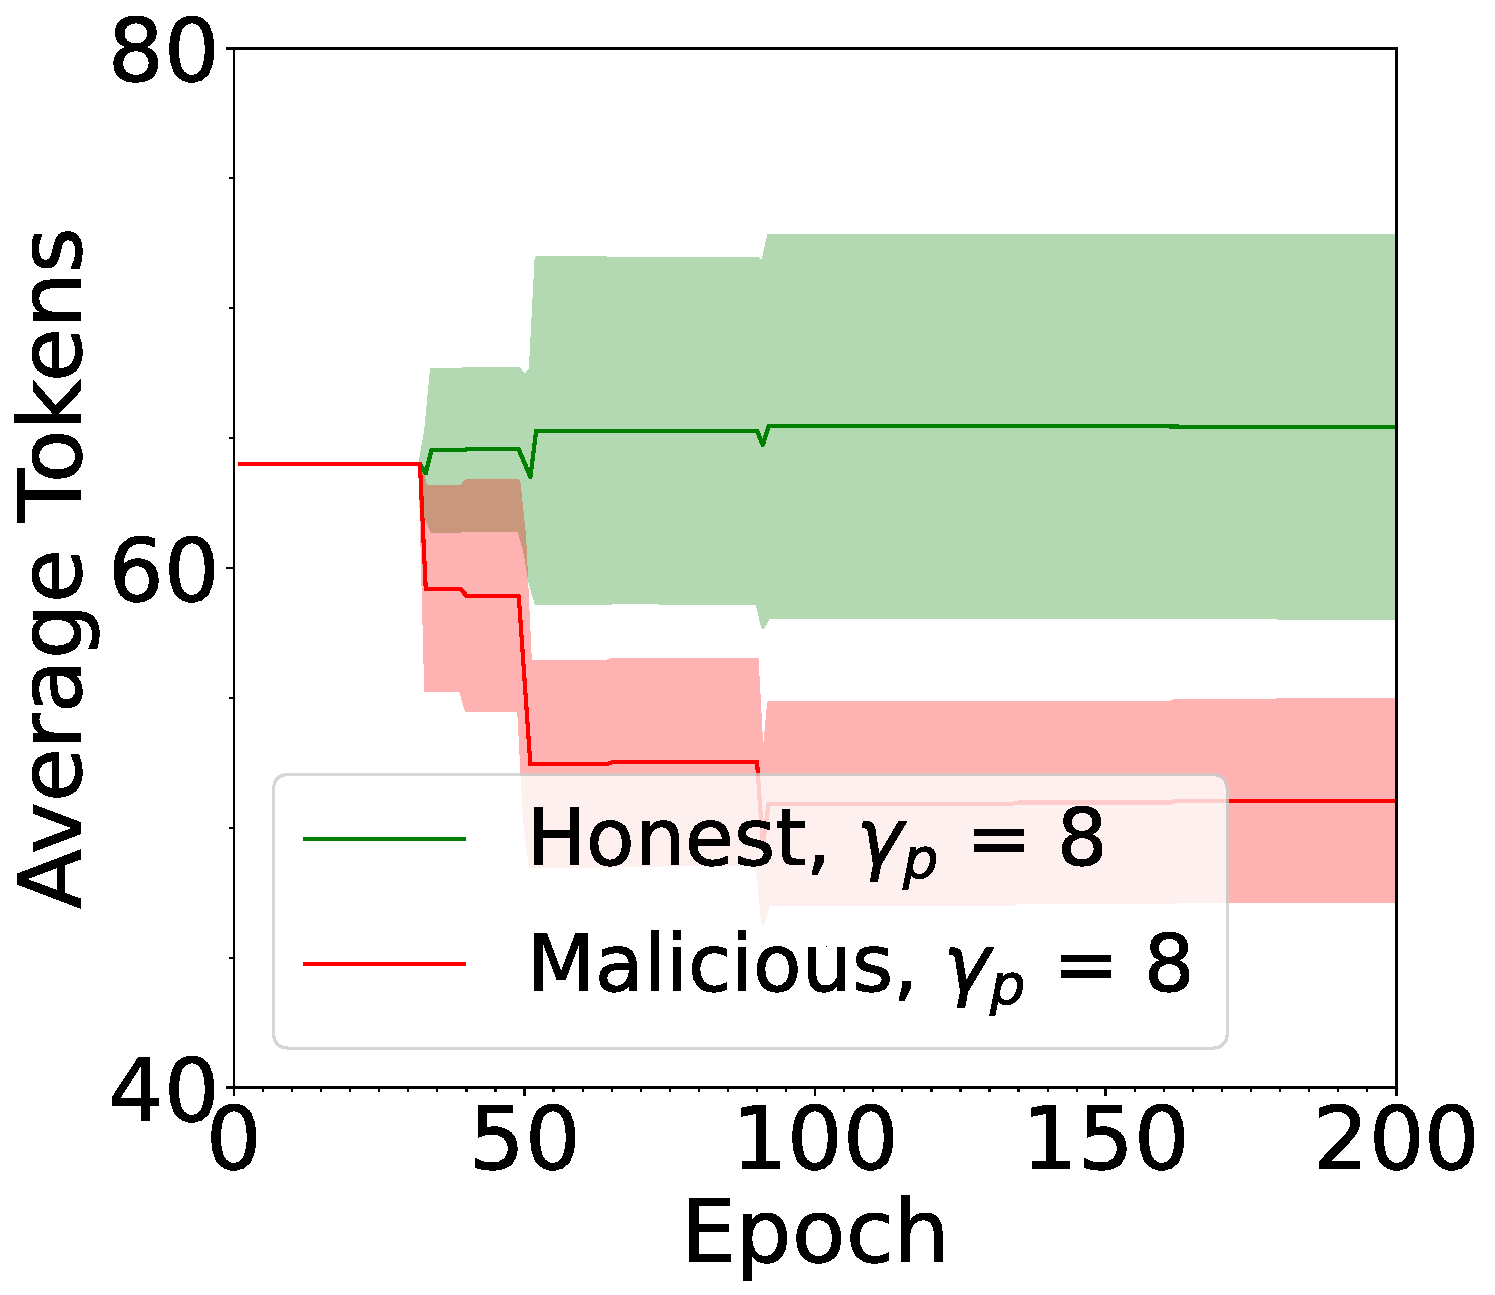
\includegraphics[width=0.483\columnwidth]{figures/tokens_with_rate_0.1.pdf}
\label{fig:tokens_with_rate_0.1}
}%
\hfill
\subfigure[$\eta$ = 0.2.]{
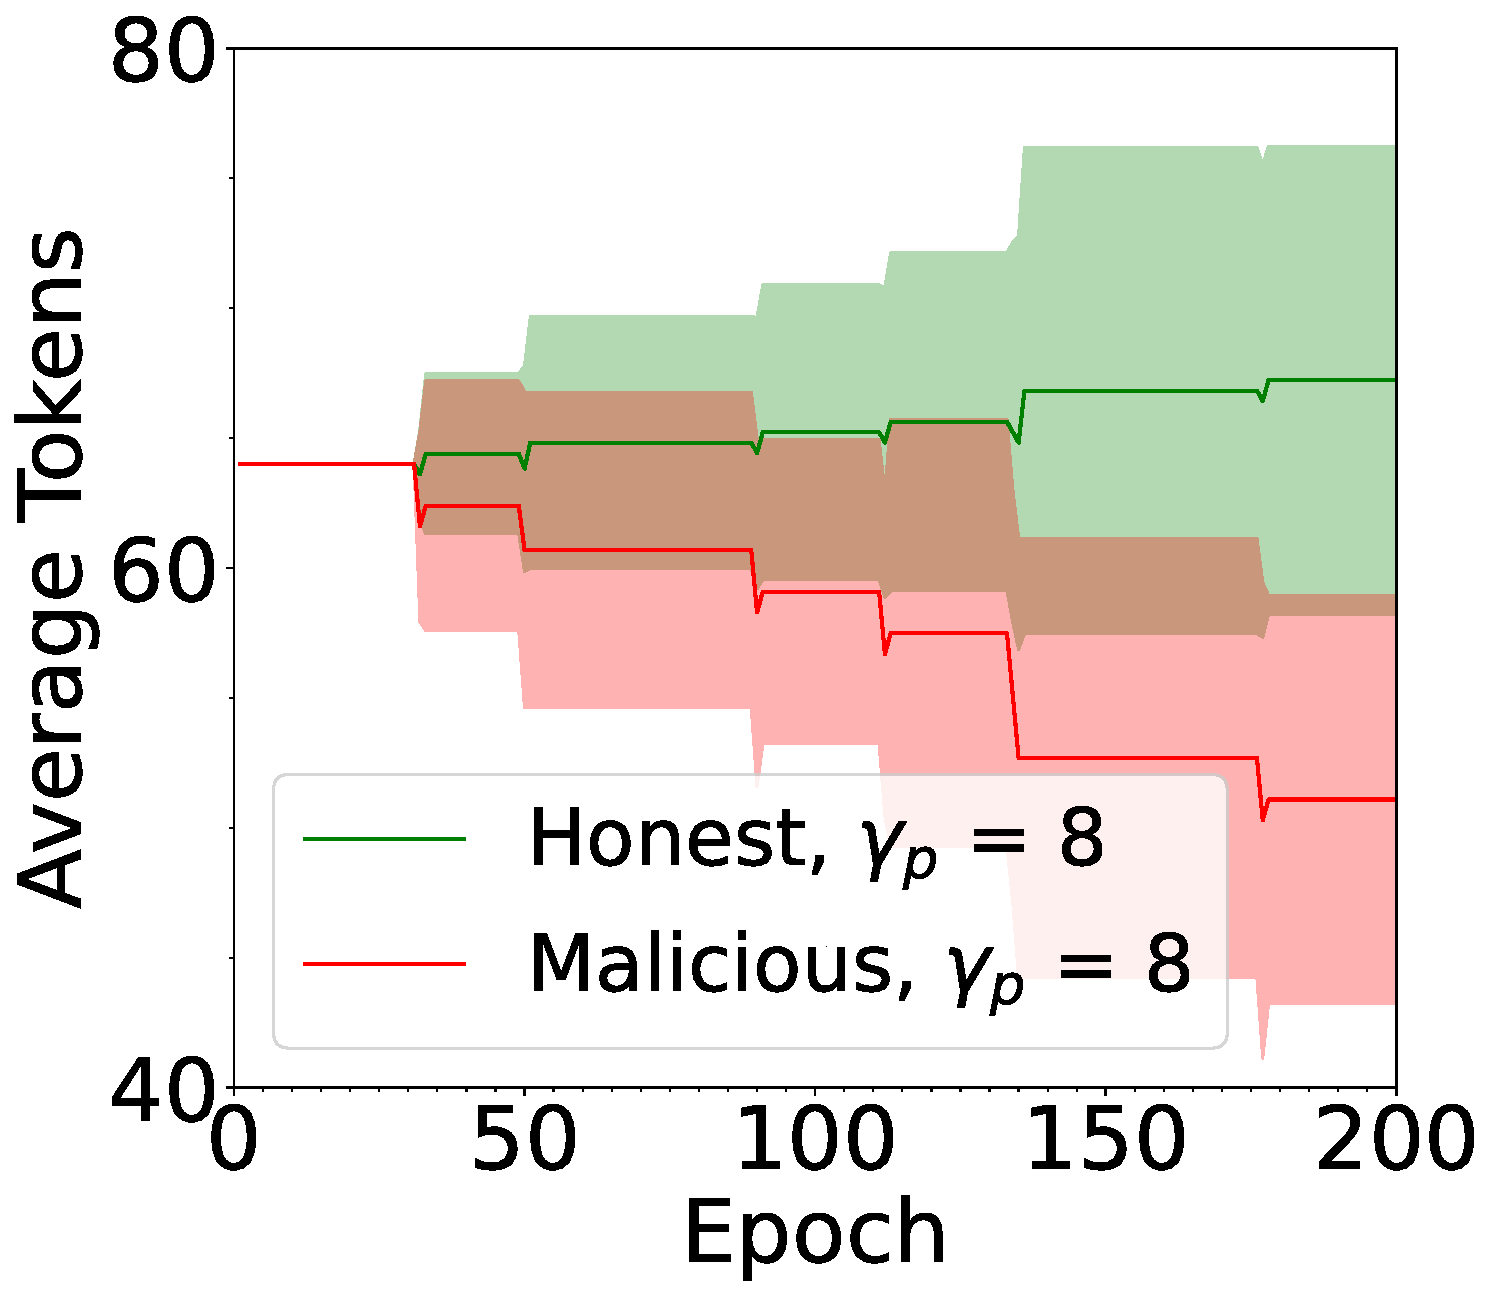
\includegraphics[width=0.483\columnwidth]{figures/tokens_with_rate_0.2.pdf}
\label{fig:tokens_with_rate_0.2}
}%
\hfill
\subfigure[$\eta$ = 0.3.]{
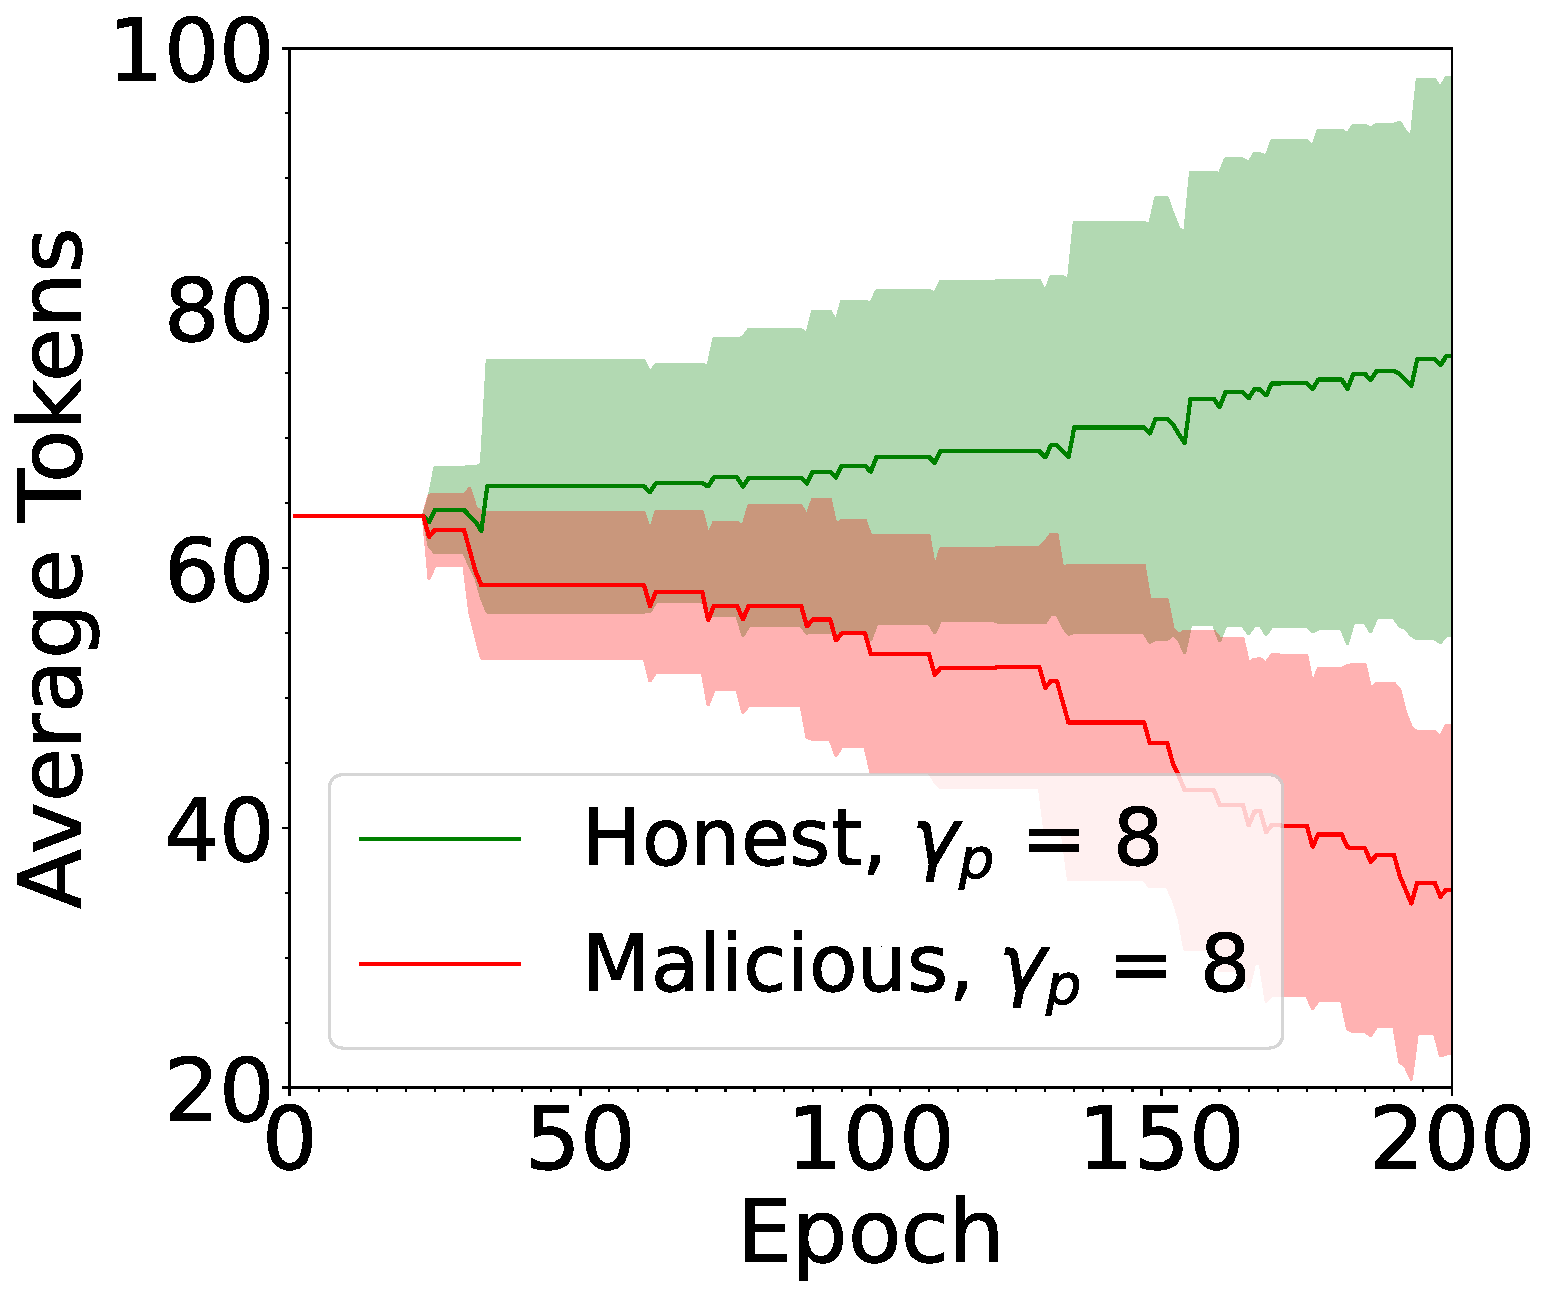
\includegraphics[width=0.483\columnwidth]{figures/tokens_with_rate_0.3.pdf}
\label{fig:tokens_with_rate_0.3}
}%
\hfill
\subfigure[$\eta$ = 0.4.]{
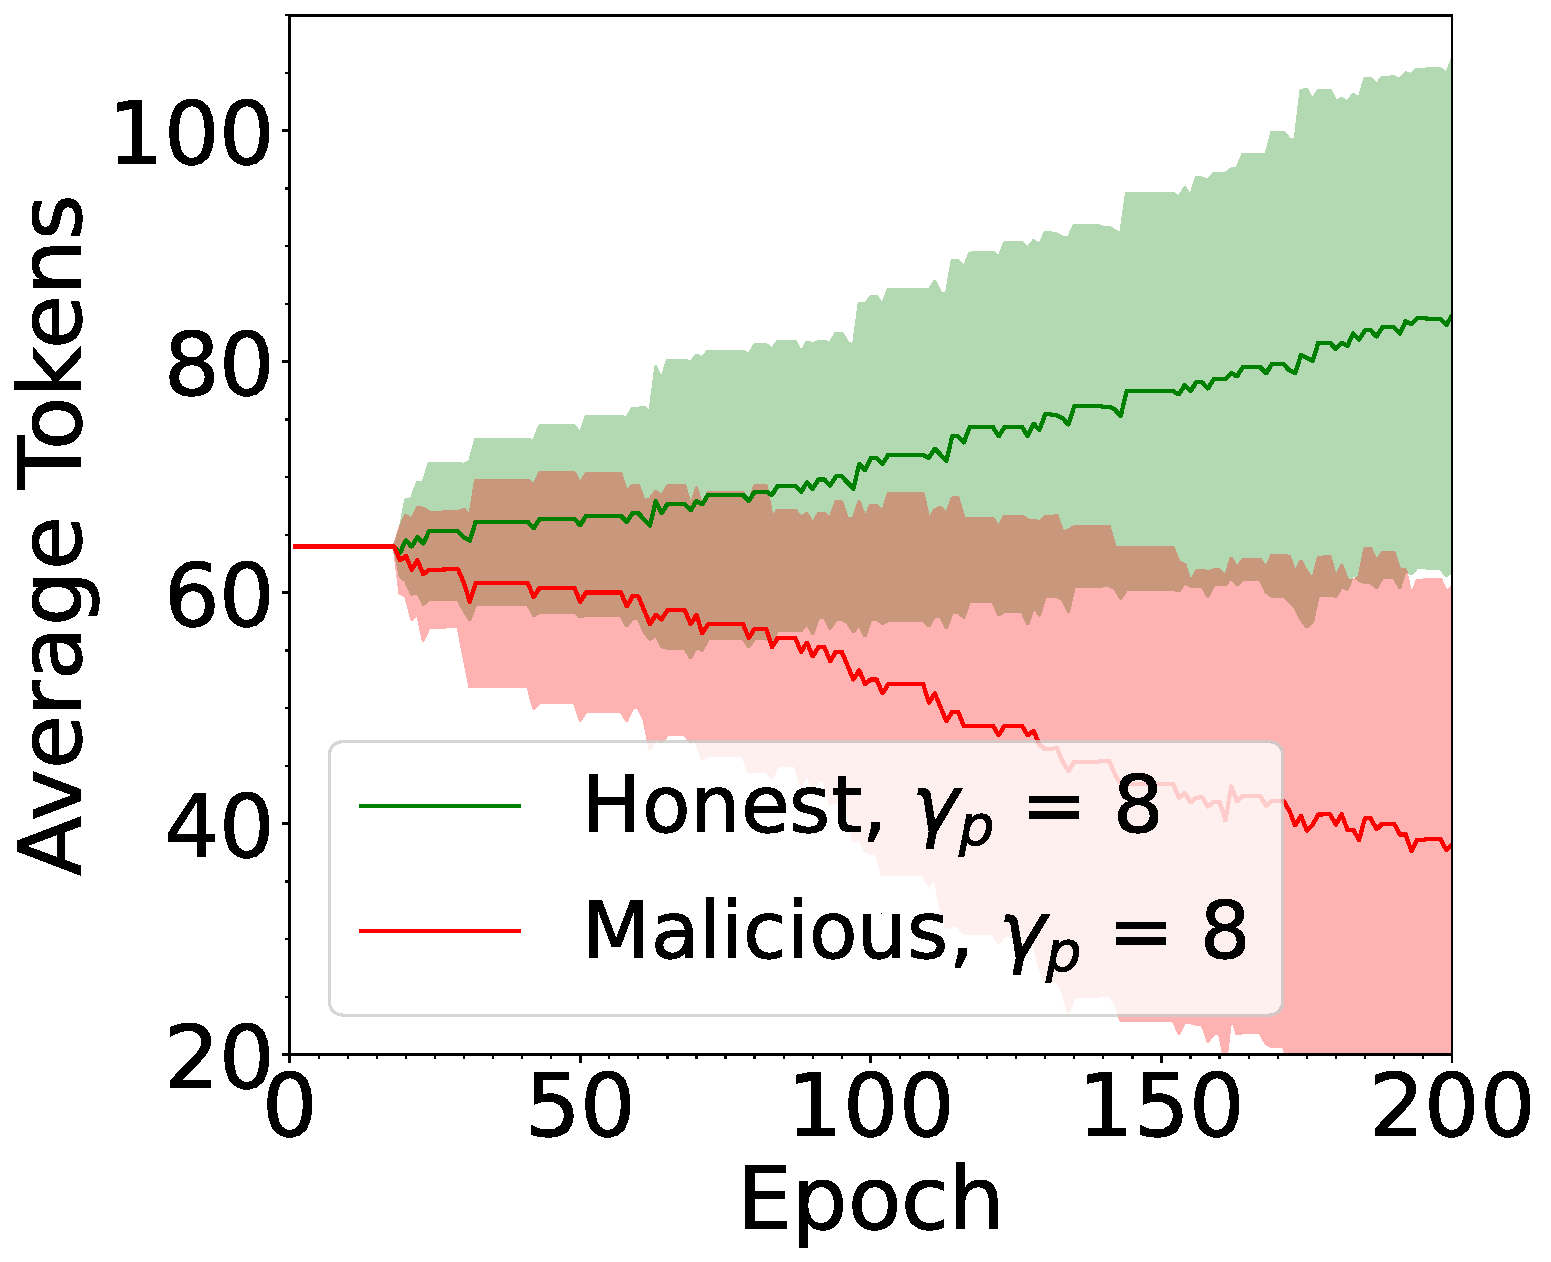
\includegraphics[width=0.483\columnwidth]{figures/tokens_with_rate_0.4.pdf}
\label{fig:tokens_with_rate_0.4}
}%
\hfill
% \vspace{-0.5cm}
\centering
\caption{Example: FL system with reward and slash mechanism  under different values of the ratio of malicious clients ($\eta$), taken from~\cite{dong2023defending}. The average balance of honest clients increases, while the average balance of malicious clients decreases over time. }
\label{fig:token_distribution_sp=8}
\end{figure*}

\subsection{\FL Validation and Voting}

\begin{itemize}
    % \item During each round $t$,  validators will download the aggregated global model $\hat{\theta^t}$. A validator $p$ assesses this model $\hat{\theta^t}$ by deploying it on their local testing dataset and generates a local validation score $s^{t}_p$, which will be used to compare with the score $s^{t-1}_p$  in the previous round, to ascertain the model's performance progression. According to the comparison results, the validator will report a voting result to the aggregator:

    \rui{\item After the model aggregation process is finalised, the voter proceeds to evaluate the aggregated model $\hat{\theta^t}$, utilising their own local testing datasets $\mathcal{D}_p^{test}$. This evaluation phase involves the computation of a local validation score, $s^{t}_p$, which functions as a criterion for assessing the model's performance. These individual validation scores are then submitted to a smart contract for aggregation. Following the aggregation, the aggregated score is compared with the previous round's score, $s^{t-1}_p$, to assess progress or decline in model performance. The smart contract then determines the next steps for the aggregated model based on these scores: advancement to the next phase for satisfactory performance improvement, or a return to the preceding validated model to begin a new cycle of training, aggregation and evaluation, if progress is deemed insufficient.
    }
    % According to the comparison results, the voter reports a voting result to the aggregator:"

\begin{equation*}
  \mathsf{vote}_p^t =
    \begin{cases}
      \phantom{+}1, & s^{t}_p \ge (1 - \epsilon) \cdot s^{t-1}_p \\
      -1, & s^{t}_p < (1 - \epsilon)\cdot  s^{t-1}_p
    \end{cases} 
\end{equation*}

Here, $\epsilon$ is a hyperparameter within the range $(0, 1)$, designated to tolerate the permissible margin of performance decline across successive rounds.

\item After receiving all reported voting results $\{\mathsf{vote}_1^t, ..., \mathsf{vote}_{P_V}^t\}$ from the validators, the aggregator will  calculate the aggregated voting result via the following formula:

\begin{equation*}
  \mathsf{aggVote}^t= \sum_{p = 1}^{ P_v}  \mathsf{vote}_p^t
\end{equation*}

For each round $t$, the finalised aggregated global model update is determined by the aggregated voting result:

\begin{equation*}
  \theta^t =
    \begin{cases}
      \hat{\theta^t}, & \mathsf{aggVote}^t \geq 0 \\
      \theta^{t-1}, & \mathsf{aggVote}^t < 0
    \end{cases} 
\end{equation*}


\end{itemize}



\subsection{\FL Rewards for Participants} The aggregated voting result $\mathsf{aggVote}^t$ will also determine the rewards distribution for participants in a \FL task.





% \begin{algorithm}[t]
%     \centering
%     \begin{algorithmic}[1]
%         \Statex $a^t$: Majority voting decision at round $t$
%         \Statex $\mathcal{K}$: Set of participating clients at round $t$
%         \Statex $\mathcal{K}_v^t$: Set of voters at round $t$
%         \Statex $\mathcal{K}_m^t$: Set of voters at round $t$ with $v_k^t == a^t$
%         \Statex $\mathsf{Bal}_k$: Asset of client $k$
%         \Statex $\gamma_v$: Staked tokens for voting
%         \Statex ${pool}_v$: Pool for storing voters' stake
%         \For{$k \in \mathcal{P}_v^t \setminus \mathcal{K}_m^t$}
%             \If {$\mathsf{Bal}_k \ge \gamma_v$}
%                 \State $\mathsf{Bal}_k \leftarrow \mathsf{Bal}_k - \gamma_v$
%                 \State ${pool}_v \leftarrow {pool}_v + \gamma_p$
%             \Else
%                 \State ${pool}_v \leftarrow {pool}_v + \mathsf{Bal}_k $
%                 \State $\mathsf{Bal}_k \leftarrow 0$
%                 \State $\mathcal{K}^t \leftarrow \mathcal{K}^t \setminus \{k\}$ 
%             \EndIf
%         \EndFor
%         \For{$k \in \mathcal{P}_m^t$}
%             \State $\mathsf{Bal}_k \leftarrow \mathsf{Bal}_k + \frac{{pool}_v}{|\mathcal{K}_m^t|} $
%         \EndFor
%         \State ${pool}_v \leftarrow  0$
%     \end{algorithmic}
%     \caption{Reward-and-slash design for \FL voters.}
%     \label{algo:2}
% \end{algorithm}




\begin{itemize}
    \item \textbf{Rewards and Penalties for Proposers/Training Nodes:} As shown in Algorithm~\ref{algo:all-fl-rewards}, in any given round $t$, should $\mathsf{aggVote}^t$ be non-negative, all training nodes selected for that round will receive rewards. Conversely, a negative aggregate vote will result in penalties for these nodes.
    
    \item \textbf{Rewards and Penalties for Voters/Validators:} As shown in Algorithm~\ref{algo:all-fl-rewards}, for round $t$, if $\mathsf{aggVote}^t \geq 0$, then validators who issued a positive vote will be rewarded, while others will face penalties. Conversely, should the aggregate vote be negative, validators who aligned with this outcome are rewarded, whereas those who did not will be penalised.
\end{itemize}





% \begin{itemize}
%     \item \textbf{Reward and Slash for Proposers/Training Nodes}: For one round $t$, if $\mathsf{aggVote}^t \geq 0$, then all selected training nodes in this round will be rewarded; otherwise, they will be slashed.

%     \item \textbf{Reward and Slash for Voters/Validators}: For one round $t$, if $\mathsf{aggVote}^t \geq 0$, then the voters/validators who reported a positive vote result will be rewarded and other voters/validators will be slashed; vice versa.

% \end{itemize}


% \
% \begin{figure*}[t]
% \centering
% \includegraphics[width=2\columnwidth]{figures/FLock-FLock-working-flow.pdf}
% \caption{FLock Workflow Overview.}
% \label{fig:FLock-FLock-working-flow}
% \end{figure*}




\subsection{Example} 
As illustrated in Figure~\ref{fig:tokens_with_rate_0.4}, taken from our previous work~\cite{dong2023defending}, proper configuration of the slashing and reward mechanisms enables the expulsion of malicious FL participants from the system, while incentivising honest behaviour. 


\subsection{\FL Improvement: ZKPs-based FL} 

FLock also adopts advanced techniques such as \ZKP~\cite{sasson2014zerocash, groth2016size} to construct secure decentralised AI training systems.

%     \begin{figure}[t]
% \centering
% 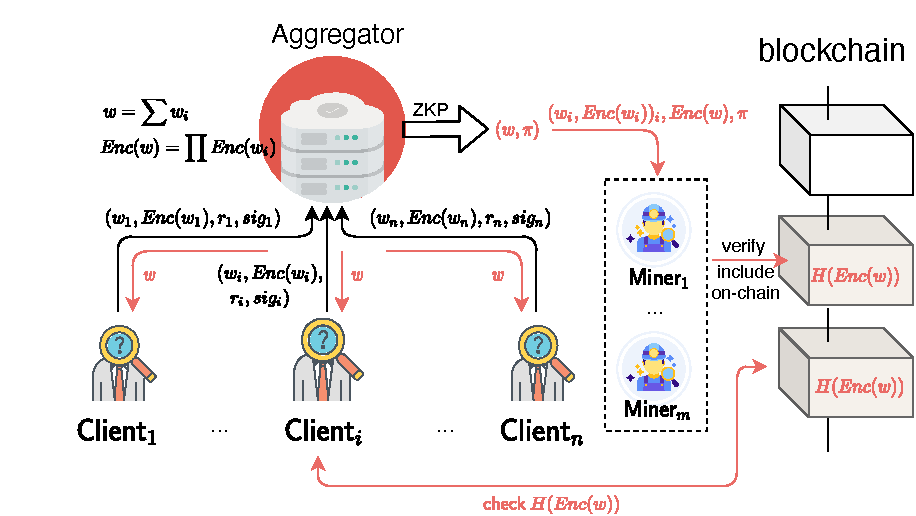
\includegraphics[width=\columnwidth]{figures/zkFL_with_blockchain.pdf}
% \caption{Overview of FL aggregation based on blockchain and ZKPs, taken from~\cite{wang2023zkfl}. }
% \label{fig:zkFL_with_blockchain}
% \end{figure}

\textit{ZKPs for \FL Aggregation:} As demonstrated in our prior study, FLock incorporates \ZKP to address the issues arising from the centralisation of the \FL aggregator/server, as detailed in our earlier research~\cite{wang2023zkfl}.  Our FL system, which can be underpinned by both blockchain technology and ZKPs and function in the following manner:

\begin{itemize}
    \item \textbf{Setup Phase:} Each participant, comprising $N$ clients and an aggregator, generates their unique private/public key pairs. These pairs are directly associated with their respective blockchain addresses.
    
    \item \textbf{Client Selection Phase:} At the beginning of each epoch, a subset of $n$ clients is selected from the total $N$ by using Verifiable Random Functions. 
    
    \item \textbf{Local Computation Phase:} The selected $n$ clients start local model training to derive their individual model updates $w_1, w_2, \ldots, w_n$. Utilising the Pedersen commitment, each client encrypts their update as $Enc(w_i) = g^{w_i}\cdot h^{s_i}$, where $g$ and $h$ are predefined public parameters and $s_i$ is a randomly generated number by the client. Following encryption, clients authenticate these updates using their private keys to produce a signature $sig_i$ and subsequently transmit the compilation of their local model update, the generated random number, the encrypted update, and the signature $(w_i, s_i, Enc(w_i), sig_i)$ to the aggregator.
    
    \item \textbf{Aggregation and ZKP Generation Phase:} The aggregator aggregates the incoming local updates to form a unified global model update $w = \sum_{i=1}^{n} {w_i}$. It also calculates the collective encrypted value of this global update as $Enc(w) = \prod_{i=1}^n Enc(w_i)$ and signs this encrypted value to produce a signature $sig$. Utilising zkSnarks, the aggregator issues a proof $\pi$ to validate the accuracy and authenticity of the aggregation process, based on the provided statement and witness, ensuring the integrity of both the individual updates and the aggregate model. Specifically, the aggregator then leverages zkSnark to issue a proof $\pi$ for the following statement and witness: 
\begin{equation*}
    \begin{cases}
      & \text{$statement = (Enc(w_1),sig_1, Enc(w_2), sig_2, $}\\
      &~~~~~~~~~~~~~~~~~~~~~~~~~\text{$..., Enc(w_n), sig_n, Enc(w))$}\\
     & \text{$witness = (w_1, s_1, w_2, s_2,..., w_n, s_n, w)$}
    \end{cases}       
\end{equation*}
% $statement = (Enc(w_1),sig_1, Enc(w_2), sig_2, ..., Enc(w_n), sig_n, Enc(w))$ ; $witness = (w_1, s_1, w_2, s_2,..., w_n, s_n, w)$ 



where the corresponding circuit $C(statement, witness)$ outputs $0$ if and only if:

\begin{equation*}
    \begin{cases}
      & \text{$\forall 1\leq i \leq n, Enc(w_i) = g^{w_i} \cdot h^{s_i}$}\\
      & \text{$w = \sum_{i=1}^{n} {w_i}$}\\
       & \text{$sig_i$ is signed by the client $i$}
    \end{cases}       
\end{equation*}
    
    \item \textbf{Global Model and Proof Dissemination Phase:} The aggregator distributes the global model update $w$ and its encryption $Enc(w)$ back to the $n$ clients. Concurrently, it broadcasts the validity proof $\pi$ along with the encrypted global model update to the block proposers.





    \item \textbf{Blockchain Verification Phase:} Upon receiving the proof $\pi$ and the encrypted global model update from the aggregator, block proposers verify $\pi$. If deemed valid, the hash of $H(Enc(w))$ is inscribed onto the blockchain, cementing the update's correctness.
    
    \item \textbf{Blockchain Consultation Phase:} As a new epoch initiates, the next cohort of $n$ selected clients peruses the blockchain to verify the inclusion of $H(Enc(w))$. Upon successful validation, they proceed with their local training, guided by the insights gleaned from the aggregated global model update $w$.
\end{itemize}

% \subsubsection{ZKPs for \FL Training}

\section{FLock Governance}

FLock token holders are entitled to engage in the system's democratised governance through a DAO. To participate in governance, token holders typically need to lock their tokens in a smart contract. Each token can represent a vote, aligning the distribution of power proportional to users' stake.  

Users can propose, debate, and vote on various aspects of  development and management, from technical updates and protocol modifications to treasury management and community initiatives. 
\begin{itemize}
    \item \textbf{Proposing:} The FLock community actively shapes the protocol's future through a proposal system for all token holders.  Proposals can range from addressing technical issues like bug fixes and algorithm optimization to driving wider community impact, such as allocating treasury funds for research or launching educational programs.
    \item \textbf{Debating:} Proposed ideas are then open for discussion and critique within the FLock community. Token holders can engage in forums, discussions, and possibly even direct communication with developers to analyze the merits and potential consequences of each proposal. This debate fosters transparency and ensures that decisions are well-informed and considered from multiple perspectives.
    \item \textbf{Voting:} Once a proposal has been sufficiently debated, token holders cast their votes to decide its fate. The voting system likely incorporates mechanisms like weighted voting (where larger holdings carry more weight) or quadratic voting (which incentivizes thoughtful contributions and discourages manipulation) to ensure fair representation.
\end{itemize}
The statement emphasizes that FLock's governance model allows for
continuous adaptation as the platform and the decentralized AI landscape evolve:

\begin{itemize}
    \item \textbf{Policy Adaptation:} As new challenges and opportunities arise, token holders can use the voting system to modify existing policies or create entirely new ones. This ensures that FLock remains relevant and responsive to the changing needs of its community and the broader AI ecosystem.
    \item \textbf{Feature Implementation:} Proposals for implementing new features can be put forward and voted on, allowing the FLock platform to grow and evolve based on user demand and feedback. This fosters innovation and keeps FLock at the forefront of decentralized AI development.
    \item \textbf{Responding to Challenges:} The ability to quickly adapt policies and implement changes allows FLock to effectively respond to unforeseen challenges like security vulnerabilities, regulatory shifts, or market fluctuations.
\end{itemize}

As FLock and decentralised AI landscape mature, token holders can adapt policies, implement new features, and respond to emerging challenges.





\section{FLock Applications}

The FLock system can be used to construct centralised AI, which have been proven to applied in the following cases.

\subsection{Decentralised AI for \LLMs}
% LLM
% 1) Pre-train: 2B. Incentivise community contribution in compute and data. If FL: unlock proprietary data that wouldn’t have been used in current open source development
% 2) fine-tune
% 2a) fine-tune crypto transaction agents: Transfer, swap, bridge, etc. (We can get Morpheus, 0xscope to host)
% 2b) fine-tune AI companions to the likes of Character.ai (we can get the likes of Character X to host)


\begin{itemize}
    \item \textbf{Pre-training of \LLMs:}
FLock facilitates the pre-training of \LLMs by leveraging a decentralised network whereby members can contribute computational resources and diverse data sets. This unlocks proprietary data that would otherwise remain inaccessible or unused in traditional, centralised open-source development. Diverse datasets ensure LLM versatility and ensures a broader representation of linguistic and cultural nuances, as well as community-defined values for \LLMs.
\item \textbf{Fine-tuning of LLMs:}
Fine-tuning involves adapting a pre-trained model to perform specific tasks or improve its accuracy on particular types of data. FLock supports fine-tuning in several ways:




\begin{itemize}
    \item \emph{Fine-tuning for Financial Transactions:} LLMs can be fine-tuned to act as intelligent agents for cryptocurrency transactions. Capabilities include transfers, swaps, and bridging between different cryptocurrencies. FLock's collaborations with platforms such as \href{https://morpheus.network/}{Morpheus Network} and \href{https://www.0xscope.com/}{0xscope} can facilitate hosting these AI models, ensuring that they are accessible and operational for the community. This enables secure and efficient AI-driven financial transactions.

 \item Fine-tuning for AI Companions: AI models can be fine-tuned to interact with users in more personalised and engaging ways, similar to those on platforms like \href{https://character.ai/}{Character.ai}. FLock can host these sophisticated AI companions, enhancing user experience through more natural and context-aware interactions.
\end{itemize}


\end{itemize}



\subsection{Decentralised AI for Stable Diffusion Models}
The FLock system can be used to fine-tune Stable Diffusion text-to-image models.  One critical component of this process involves Low-Rank Adaptation (LoRA)~\cite{hu2021lora}, which modifies certain parameters within the model's architecture to make it more adaptable to specific tasks without extensive retraining.

\begin{itemize}
    \item \textbf{Fine-tuning LoRA:} LoRA is designed to adapt pre-trained models by introducing trainable low-rank matrices into the architecture. This technique allows for efficient adaptation with minimal additional computational cost and a smaller number of trainable parameters. In the context of FLock and Stable Diffusion Models, applying LoRA is particularly advantageous for several reasons:
\begin{itemize}
    \item \emph{Community-Driven Enhancements:} By decentralising the fine-tuning process, FLock broadens participation in contributing specific knowledge and preferences. Artists, designers, and other creatives can input unique styles or features they wish to see enhanced, improving output quality and ensuring that it serves a wider array of cultural contexts and artistic expressions.

 \item \emph{Scalability and Accessibility:} Fine-tuning with LoRA can be scaled across multiple nodes, facilitating more widespread and continuously iterative improvements.

 \item \emph{Use Case Expansion:} By fine-tuning Stable Diffusion Models with LoRA, FLock can cater to specific industries or niches. For example, the model could be fine-tuned to generate medical illustrations for educational purposes, architectural visualisations for real estate, or unique art styles for digital media.

\end{itemize}
\end{itemize}





\subsection{Decentralised AI for Linear Regression Models}
% 1) Healthcare/ diabetes use case with FL

Linear regression models~\cite{montgomery2021introduction} are fundamental tools in statistical analysis and predictive modeling, widely used for their simplicity and effectiveness in understanding relationships between variables. FLock applies these principles in a decentralised setting to address specific healthcare challenges, such as diabetes management.


Diabetes management presents a critical area where linear regression can be effectively utilised to predict patient outcomes based on various inputs such as blood sugar levels, diet, exercise, and medication adherence. \FL facilitates the development of these predictive models with decentralised data sources in a way that respects patient data protection.


\begin{itemize}
    \item \emph{Data Protection and Security:} FLock allows multiple healthcare providers to collaborate in the model training process without actually sharing the data. This method is crucial for complying with stringent health data protection regulations such as HIPAA in the U.S. Each participant (e.g., hospitals, and clinics) retains control over their data, which is used to compute model updates locally. These updates are then aggregated to improve a shared model without exposing individual patient data.

\item \emph{Enhanced Model Accuracy and Reliability:} By integrating data from a diverse range of demographics and geographical locations, FLock can help develop more accurate and generalised linear regression models for diabetes management. This diversity is especially important in healthcare, where patient populations can vary significantly, affecting the reliability of predictive models.

\item \emph{Collaborative Innovation:} Different healthcare entities contribute to a common goal, accelerating innovation and leading to the discovery of novel insights into diabetes management and treatment strategies.
\end{itemize}


% \subsection{FLock in Finance + AI}
% \subsection{FLock in Medeical + AI}


% \subsection{Specialised Autonomous Agents}
% LLM finetuning, multi agents, GPTResearcher 



% 2. SD
% 1) fine-tune LoRA
% 3. Linear regression models
% 1) Healthcare/ diabetes use case




\section{Conclusion}
FLock provides solutions to build decentralised AI through \SNT, \FL, and AI Marketplace. FLock dismantles obstacles that hinder participation in AI systems, enabling developers to contribute models, data, or computational resources in a flexible, modular fashion. FLock fosters the creation of a diverse array of models, meticulously crafted by and expressly for the communities they serve in AI models.







\bibliography{references}
\bibliographystyle{IEEEtran}

% \clearpage

% \begin{sidewaysfigure}
%     \centering
%     \includegraphics[width=\columnwidth]{figures/FLock-FLock-working-flow.pdf}
% \caption{FLock Workflow Overview.}
% \label{fig:FLock-FLock-working-flow}
% \end{sidewaysfigure} 


\end{document}
